\documentclass[mat1, tisk]{fmfdelo}
% \documentclass[fin1, tisk]{fmfdelo}
% Če pobrišete možnost tisk, bodo povezave obarvane,
% na začetku pa ne bo praznih strani po naslovu, …

%%%%%%%%%%%%%%%%%%%%%%%%%%%%%%%%%%%%%%%%%%%%%%%%%%%%%%%%%%%%%%%%%%%%%%%%%%%%%%%
% METAPODATKI
%%%%%%%%%%%%%%%%%%%%%%%%%%%%%%%%%%%%%%%%%%%%%%%%%%%%%%%%%%%%%%%%%%%%%%%%%%%%%%%

% - vaše ime
\avtor{Matej Novoselec}

% - naslov dela v slovenščini
\naslov{Schwarzov princip zrcaljenja za harmonične funkcije}

% - naslov dela v angleščini
\title{Schwarz Reflection Principle for Harmonic Functions}

% - ime mentorja/mentorice s polnim nazivom:
%   - doc.~dr.~Ime Priimek
%   - izr.~prof.~dr.~Ime Priimek
%   - prof.~dr.~Ime Priimek
%   za druge variante uporabite ustrezne ukaze
%\mentor{prof. dr. Barbara Drinovec Drnovšek}
% \somentor{...}
\mentorica{prof. dr. Barbara Drinovec Drnovšek}
% \somentorica{...}
% \mentorja{...}{...}
% \somentorja{...}{...}
% \mentorici{...}{...}
% \somentorici{...}{...}

% - leto diplome
\letnica{2023} 

% - povzetek v slovenščini
%   V povzetku na kratko opišite vsebinske rezultate dela. Sem ne sodi razlaga
%   organizacije dela, torej v katerem razdelku je kaj, pač pa le opis vsebine.
\povzetek{

    Realne harmonične funkcije dveh realnih oziroma ene kompleksne spremenljivke lahko smatramo kot realne dele holomorfnih funkcij. 
    Pristop je koristen pri obravnavi lastnosti harmoničnih funkcij.
    Tako se na primer lastnost povprečne vrednosti in gladkost holomorfnih funkcij preneseta na harmonične funkcije. 
    Spoznamo, da tako kot za holomorfne tudi za harmonične funkcije velja princip maksima.
    
    Od obravnave prek holomorfnih funkcij se nekoliko oddaljimo pri formulaciji in reševanju Dirichletovega problema za enotski disk. 
    Problem najprej rešimo za preproste zvezne funkcije. 
    Rešitev za splošno zvezno funkcijo iščemo s pomočjo intuitivno izpeljanih zapisov pri enostavnih primerih. 
    Tako vpeljemo pojem Poissonovega jedra in Poissonovega integrala. 
    Natančneje spoznamo nekaj lastnosti vsakega izmed pojmom in izpeljemo Schwarzovo integralsko formulo. 
    Prek Poissonovega integrala nato rešimo zastavljen Dirichletov problem za enotski disk.

    Rešitev Dirichletovega problema nam priskoči na pomoč pri dokazu karakterizacije harmoničnih funkcij z lastnostjo povprečne vrednosti. 
    Omenjeno karakterizacijo lahko primerjamo s karakterizacijo holomorfnih funkcij prek izreka Morera. 
    Karakterizaciji uporabimo pri dokazu Schwarzovega principa zrcaljenja za harmonične oziroma holomorfne funkcije.

}

% - povzetek v angleščini
\abstract{

    Harmonic functions of two real or one complex variable can be viewed as real parts of holomorphic functions.
    Approach is useful when we want to study properties of harmonic functions.
    Mentioned approach lets us prove, that the mean value property and the smoothness of holomorphic functions are transferred to harmonic functions.
    We also show, that maximum principle holds for harmonic functions as it holds for holomorphic functions.

    We step away from study of holomorphic functions to formulate and solve Dirichlet problem for unit disk.
    First we solve the problem for simple continuous functions.
    In search for solution in general case, we look into intuitively derived notations for simple cases.
    Thus we introduce the concept of Poisson kernel and Poisson integral.
    We investigate some properties of each concept and prove Schwarz's integral formula.
    Using Poisson integral we then solve Dirichlet problem for unit disk in general case. 

    Solution of the Dirichlet problem helps us prove the characterization of harmonic functions with the mean value property.
    Mentioned characterization is similar to the characterization of holomorphic functions through Morera's theorem.
    We exploit characterizations to prove Schwarz reflection principle for harmonic and holomorphic functions respectively.

}

% - klasifikacijske oznake, ločene z vejicami
%   Oznake, ki opisujejo področje dela, so dostopne na strani https://www.ams.org/msc/
\klasifikacija{..., ...}

% - ključne besede, ki nastopajo v delu, ločene s \sep
\kljucnebesede{harmonična funkcija\sep
    Laplaceov operator\sep
    območje\sep
    enotski disk\sep
    lastnost povprečne vrednosti\sep
    princip maksima\sep
    Dirichletov problem\sep
    Poissonovo jedro\sep
    Poissonov integral\sep
    razširitev\sep
    Schwarzov princip zrcaljenja}

% - angleški prevod ključnih besed
\keywords{harmonic function\sep
    Laplace operator\sep
    domain\sep
    unit disk\sep
    mean value property\sep
    maximum principle\sep
    Dirichlet problem\sep
    Poisson kernel\sep
    Poisson integral\sep
    extenstion\sep
    Schwarz reflection principle} 

% - angleško-slovenski slovar strokovnih izrazov
\slovar{

\geslo{harmonic function}{harmonična funkcija}
\geslo{holomorphic function}{holomorfna funkcija}
\geslo{Cauchy-Riemann system of equations}{Cauchy-Riemann sistem enačb}
\geslo{domain}{območje}
\geslo{boundary}{rob}
\geslo{mean value property}{lastnost povprečne vrednosti}
\geslo{maximum principle}{princip maksima}
\geslo{Dirichlet problem for unit disk}{Dirichletov problem za enotski disk}
\geslo{Poisson kernel}{Poissonovo jedro}
\geslo{Poisson integral}{Poissonov integral}
\geslo{Schwarz reflection principle}{Schwarzov princip zrcaljenja}
\geslo{reflection of domain over real axis}{zrcalna slika območja glede na realno os}
\geslo{extension of function}{razširitev funkcije}

}

% - ime datoteke z viri (vključno s končnico .bib), če uporabljate BibTeX
% \literatura{....bib}

%%%%%%%%%%%%%%%%%%%%%%%%%%%%%%%%%%%%%%%%%%%%%%%%%%%%%%%%%%%%%%%%%%%%%%%%%%%%%%%
% DODATNE DEFINICIJE
%%%%%%%%%%%%%%%%%%%%%%%%%%%%%%%%%%%%%%%%%%%%%%%%%%%%%%%%%%%%%%%%%%%%%%%%%%%%%%%

% naložite dodatne pakete, ki jih potrebujete
% \usepackage{...}
\usepackage{graphicx}
\usepackage{amsmath}
\usepackage{yhmath}
\usepackage{float}
\usepackage[shortlabels]{enumitem}
\usepackage[justification=centering]{caption}

% deklarirajte vse matematične operatorje, da jih bo LaTeX pravilno stavil
% \DeclareMathOperator{\...}{...}

% vstavite svoje definicije ...
% \newcommand{\...}{...}
\newcommand{\R}{\mathbb R}
\newcommand{\N}{\mathbb N}
\newcommand{\Z}{\mathbb Z}
\newcommand{\C}{\mathbb C}
\newcommand{\Q}{\mathbb Q}

%%%%%%%%%%%%%%%%%%%%%%%%%%%%%%%%%%%%%%%%%%%%%%%%%%%%%%%%%%%%%%%%%%%%%%%%%%%%%%%
% ZAČETEK VSEBINE
%%%%%%%%%%%%%%%%%%%%%%%%%%%%%%%%%%%%%%%%%%%%%%%%%%%%%%%%%%%%%%%%%%%%%%%%%%%%%%%

\begin{document}

\section{Uvod}

Dotični matematični objekt diplomske naloge bodo harmonične funkcije. 
Kot rešitve Laplaceove parcialne diferencialne enačbe igrajo pomembno vlogo v številnih področjih matematike, predvsem kompleksni in harmonični analizi, fiziki ter inženirstvu. 
Ena izmed glavnih matematičnih motivacij za preučevanje harmoničnih funkcij, se skriva v dejstvu, da lahko realne harmonične funkcije dveh realnih spremenljivk obravnavamo kot realni del holomorfne funkcije.
Cilj diplomskega dela je za omenjen razred funkcij dokazati Schwarzov princip zrcaljenja.
Zasluge za izrek so, kot to že nakazuje samo ime, pripisane nemškemu matematiku Hermannu Schwarzu.
Izrek igra pomembno vlogo predvsem pri razumevanju obnašanja harmoničnih funkcij na območjih v kompleksni ravnini. 
Njegove posplošitve, zapisane v zaključku diplomskega dela, pa so pomembno orodje za vzpostavljanje povezav med različnimi območji v kompleksni ravnini.

Začetna poglavja diplomskega dela omogočajo uporabo spoznanih pojmov in dejstev v šestim poglavju, ter z njim tvorijo smiselno celoto.
V drugem poglavju bomo spoznali nekatere osnovne lastnosti harmoničnih funkcij, tretje poglavje pa je namenjeno vpeljavi pojma lastnosti povprečne vrednosti. 
Spoznali bomo, da je omenjena lastnost ena ključnih za preučevanje harmoničnih funkcij. 
Sledi četrto poglavje, katerega vsebina se bo na prvi pogled nekoliko oddaljila od naslova diplomskega dela. 
Poglavje je namenjeno obravnavi pojmov, ki nas bodo pripeljali do rešitve Dirichletovega problema za enotski disk.
V zadnjem razdelku poglavja bo delo poplačano. Rešen Dirichletov problem za enotski disk bomo uporabili za dokaz karakterizacije harmoničnih funkcij prek lastnosti povprečne vrednosti.
Ta nam bo v petem poglavju omogočala dokaz glavnega izreka. 

%------------------------------------------------------------
\section{Harmonične funkcije}

Začetek poglavja je namenjen ponovitvi znanih pojmov, konec pa zapisu glavnih lastnosti na katere se bomo kasneje sklicevali. 

\subsection{Osnovni pojmi}

    Navedimo nekaj osnovnih definicij in komentarjev. 

    \begin{definicija}
        \label{harm}
        Naj bo $U$ odprta podmnožica v $\mathbb{R}^n$. Naj bo $u$ funkcija, definirana na $U$ in naj bo na definicijskem območju dvakrat zvezno odvedljiva.  
        Pravimo, da je funkcija $u(x_1, x_2, \dots, x_n)$ \emph{harmonična}, če velja
        $$
        \frac{\partial^2 u}{\partial x_1 ^ 2} +  \frac{\partial^2 u}{\partial x_2 ^ 2} + \dots + \frac{\partial^2 u}{\partial x_n ^ 2} = 0.
        $$
        Operatorju $\Delta  = \frac{\partial^2}{\partial x_1 ^ 2} +  \frac{\partial^2}{\partial x_2 ^ 2} + \dots + \frac{\partial^2}{\partial x_n ^ 2}$ pravimo \emph{Laplaceov operator} in pišemo
        $$
        \Delta u = 0.
        $$
    \end{definicija}

    Pogoj za harmoničnost podaja Laplaceovo parcialno diferencialno enačbo, zapisano bodisi s Laplaceovim operatorjem ali razpisano s parcialnimi odvodi drugega reda. 
    Funkcija je torej harmonična, če zadošča zgoraj zapisani parcialni diferencialni enačbi. 

    Vredno je omeniti, da v zgornji definiciji nismo specificirali, ali gre pri funkciji $u$ za realno ali kompleksno funkcijo. 
    Pojem harmoničnosti smo definirali v splošnem, torej tako za kompleksne kot tudi realne funkcije.
    Znotraj diplomske naloge se bomo omejili na funkcije dveh realnih spremenljivk ali funkcijo ene kompleksne spremenljivke. To bomo nato velikokrat delili na realni in imaginarni del ($z = x + iy $) in na ta način prešli nazaj na funkcije dveh realnih spremenljivk.
    Pogoj za harmoničnost takrat zapišemo kot
        $$
            \Delta u = \frac{\partial^2 u}{\partial x ^ 2} +  \frac{\partial^2 u}{\partial y ^ 2}= 0.
        $$

    \begin{definicija}
        \emph{Območje} $D$ je povezana odprta podmnožica v $\mathbb{C}$.
        Če obstaja $a \in D$, da za vse $b \in D$ in vse $t \in [0,~1]$ tudi $t a + (1-t)b \in D$ pravimo, da je $D$ \emph{zvezdasto območje}.
    \end{definicija}

\subsection{Lastnosti harmoničnih funkcij}

    S pomočjo orodij iz kompleksne analize se lotimo obravnave osnovnih lastnosti. 

    \begin{trditev}
        \label{hh}
        Naj bo $U \subseteq \mathbb{C}$ odprta množica. Naj bo $f = u + iv$ holomorfna funkcija, $u$ in $v$ pa realni funkciji, definirani na $U$. Potem sta funkciji $u$ in $v$ na $U$ harmonični.
    \end{trditev}

    \begin{dokaz}
        Ker je $f$ holomorfna, zadošča Cauchy-Riemannovemu sistemu enačb. Sledi
        \begin{align*}
            \frac{\partial^2 u}{\partial x^2} &= \frac{\partial^2 v}{\partial x \partial y}~~~~\text{in}~~~~\frac{\partial^2 u}{\partial x \partial y} = \frac{\partial^2 v}{\partial y^2}~,~~\text{ter}\\ 
            \frac{\partial^2 u}{\partial y^2} &=  - \frac{\partial^2 v}{\partial x \partial y}~~~~\text{in}~~~~\frac{\partial^2 u}{\partial x \partial y} =  - \frac{\partial^2 v}{\partial x^2}.
        \end{align*}
        Zato velja $\frac{\partial^2 u}{\partial x^2} + \frac{\partial^2 u}{\partial y^2} = \frac{\partial^2 v}{\partial x \partial y} - \frac{\partial^2 v}{\partial x \partial y} =0$ in $\frac{\partial^2 v}{\partial x^2} + \frac{\partial^2 v}{\partial y^2} = \frac{\partial^2 u}{\partial x \partial y} - \frac{\partial^2 u}{\partial x \partial y}=0$.
    \end{dokaz}

    \begin{opomba}
        Če označimo $u = \text{Re}[f]$ in $v = \text{Im}[f]$, nam zgornja trditev pove, da sta realni in imaginarni del holomorfne funkcije harmonični funkciji. 
    \end{opomba}

    \begin{definicija}
        Naj bo $u$ realna harmonična funkcija, definirana na območju $D$. Če obstaja realna harmonična funkcija $v$, definirana na $D$, da je funkcija $f = u + iv$ na $D$ holomorfna, potem funkciji $v$ pravimo \emph{harmonična konjugiranka funkcije $u$ na $D$}.    
    \end{definicija}

    \begin{trditev}
        \label{konj}
        Naj bo $u$ realna harmonična funkcija, definirana na zvezdastem območju $D$. Potem za $u$ na $D$ obstaja harmonična konjugiranka $v$ in je do konstante natančno enolično določena. 
    \end{trditev}
    \begin{dokaz}
        Konstrukcijo harmonične konjugiranke si bralec, za primer ko je zvezdasto območje kar odprt disk, lahko ogleda v \cite{osnova} na strani $56$ in $57$. 
        Ideja dokaza za splošno zvezdasto območje je podobna. 
    \end{dokaz}

    V duhu trditev \ref{hh} in \ref{konj}, je velikokrat smiselno na realno harmonično funkcijo $u$ gledati kot na realni del holomorfne funkcije $f = u + iv$, kjer je $v$ njena harmonična konjugiranka. To že nakazuje, da se bodo nekatere lepe lastnosti holomorfnih funkcij prenesle tudi na harmonične funkcije.
    Opazimo tudi, da je zaradi linearnosti parcialnih odvodov, tudi linearna kombinacija harmoničnih funkcij harmonična. To bomo pri reševanju enega izmed glavnih problemov diplomskega dela s pridom uporabili.

    \begin{opomba}
        V literaturi se v definiciji harmoničnosti, za funkcijo $u$, pojavlja tudi zahteva, da je funkcija gladka oziroma $u \in C^{\infty}$. V zgornji definiciji zahtevamo le obstoj drugih parcialnih odvodov, oziroma $u \in C^2$. 
        Da sta definiciji za realne funkcije dveh spremenljivk med seboj ekvivalentni, potrdi spodnja trditev. 
    \end{opomba}
    \begin{trditev}
        \label{gladkost_re_h}
        Naj bo $u$ realna harmonična funkcija, definirana na območju $D$. Potem je $u$ na $D$ gladka, oziroma $u \in C^{\infty}(D)$. 
    \end{trditev}
    \begin{dokaz}
        Ker je  $D$ odprta množica, lahko za vsako točko $z \in D$ najdemo dovolj majhno zvezdasto okolico $U_z$, da bo okolica v celoti vsebovana v $D$. Dovolj je vzeti kar dovolj majhen disk. 
        Po trditvi \ref{konj} na $U_z$ obstaja harmonična konjugiranka $v$, da je $f = u+ iv$ na $U_z$ holomorfna, ter zato na $U_z$ tudi gladka. Sledi, da je na $U_z$ gladka tudi funkcija $u$.
        Ker smo za vsako točko iz $D$ našli odprto okolico, na kateri je funkcija $u$ gladka, je $u$ gladka na celotnem definicijskem območju.
    \end{dokaz}
    \begin{posledica}
        \label{gladkost_komp_h}
        Naj bo $u$ kompleksna harmonična funkcija, definirana na območju $D$. Potem je $u$ na $D$ gladka, oziroma $u \in C^{\infty}(D)$. 
    \end{posledica}
    \begin{dokaz}
        Označimo $u = u_1 + i u_2$, kjer sta $u_1$ in $u_2$ realni harmonični funkciji, definirani na $D$. Po trditvi \ref{gladkost_re_h} sta $u_1$ in $u_2$ gladki na $D$, zato je na $D$ gladka tudi funkcija $u$.
    \end{dokaz}

    \begin{trditev}
        \label{komp_s_hol}
        Naj bo $u$ realna harmonična funkcija, definirana na območju $D$. Naj bo $\Omega$ območje in $f : \Omega \to D$ holomorfna funkcija. Potem je $u \circ f$ na $\Omega$ harmonična funkcija.
    \end{trditev}
    \begin{dokaz}
        Naj bo $z_0$ poljubna točka iz $\Omega$. Dovolj je pokazati, da ima $z_0$ odprto okolico, na kateri je $u \circ f$ harmonična. Ker je $D$ območje, obstaja $r > 0$, da je \mbox{$\mathbb{D}(f(z_0), r) \subseteq D$}. 
        Po trditvi \ref{konj} zato za $u$ na $\mathbb{D}(f(z_0),r)$ obstaja $v$, da je $g = u + iv$ na $\mathbb{D}(f(z_0), r)$ holomorfna. Sledi, da je $g \circ f$ holomorfna na $\left\{z~|~ f(z) \in \mathbb{D}(f(z_0), r)\right\}$.
        Ker je $f$ holomorfna, je $A_{z_0} = \left\{z~|~ f(z) \in \mathbb{D}(f(z_0), r)\right\}$ odprta okolica za $z_0$. Po trditvi \ref{hh} je na odprti okolici $A_{z_0} \subseteq \Omega$, točke $z_0$ funkcija $\text{Re}[g \circ f] = \text{Re}[(u + iv)\circ f] = \text{Re}[(u \circ f) + i(v \circ f)] = u \circ f$ harmonična. 
        Zato je $u \circ f$ harmonična na $\Omega$.
    \end{dokaz}

    \begin{posledica}
        \label{komp_s_hol_komp}
        Naj bo $g$ kompleksna harmonična funkcija, definirana na območju $D$. Naj bo $\Omega$ območje in $f : \Omega \to D$ holomorfna funkcija. Potem je $g \circ f$ na $\Omega$ harmonična funkcija.
    \end{posledica}
    \begin{dokaz}
        Zapišimo $g = u_1 + i u_2$, kjer sta $u_1$ in $u_2$ realni funkciji, definirani na $D$. 
        Ker je $g$ harmonična, velja $ 0 = \Delta g = \Delta(u_1 + i u_2) = \Delta u_1 + i \Delta u_2$. Sledi $\Delta u_1 = \Delta u_2 = 0$, oziroma $u_1$ in $u_2$ sta realni harmonični funkciji.
        Trditev \ref{komp_s_hol} nam pove, da sta potem funkciji $u_1 \circ f$ in $u_2 \circ f$ harmonični na $D$. Zaradi linearnosti Laplaceovega operatorja lahko zaključimo, da je potem na $D$ harmonična tudi funkcija $(u_1 \circ f) + i (u_2 \circ f) = (u_1 + i u_2) \circ f = g \circ f$.
    \end{dokaz}

\section{Lastnost povprečne vrednosti}

Na prvi pogled se bodo pojmi, obravnavani v začetku poglavja, zdeli nepovezani s študijo harmoničnih funkcij. Povezava bo razvidna iz drugega razdelka poglavja.

\subsection{Definicija in osnovne lastnosti}

    Za začetek le navedimo definicijo in zapišimo nekaj opazk.

    \begin{definicija}  
        Naj bo $h$ kompleksna zvezna funkcija, definirana na območju $D$. Denimo, da za $z_0 \in D$ in $r_0 > 0$ velja $\overline{\mathbb{D}}(z_0, r_0) \subseteq D$. \emph{Povprečje funkcije} $h$ na $\overline{\mathbb{D}}(z_0, r_0)$ definiramo kot
        $$
            A(r) = \int_{0}^{2 \pi}{h \big(z_0 + r e^{i\theta}\big)\frac{d\theta}{2 \pi}}~,~~\text{za}~~r \in (0,r_0].
        $$
    \end{definicija}
    \begin{trditev}
        \label{zvpov}
        Naj bo $h$ kompleksna zvezna funkcija, definirana na območju $D$, ter denimo, da za $z_0 \in D$ in $r_0 > 0$ velja $\overline{\mathbb{D}}(z_0, r_0) \subseteq D$. 
        Potem je funkcija $A$ zvezna na $(0,~r_0]$ in velja $\lim_{r \downarrow 0}{A(r)} = h(z_0)$.
    \end{trditev}
    \begin{dokaz}
        Ker je povprečje zvezne funkcije definirano kot integral zvezne funkcije, je funkcija $A$ zvezna na $(0,~r_0]$. Drugi del trditve dokažimo po definiciji.
        Naj bo $\epsilon > 0$ poljubno majhen. Velja
        $$
            |A(r) - h(z_0)| = \bigg|\int_{0}^{2\pi} \left(h(z_0 + r e^{i\theta})  - h(z_0)\right) \frac{d\theta}{2\pi} \bigg| \leq \int_{0}^{2 \pi} \big| h(z_0 + r e^{i\theta}) - h(z_0) \big| \frac{d\theta}{2 \pi}.
        $$
        Ker je $h$ zvezna, obstaja $\delta > 0$, da za vsak $r \in  (0,~\delta)$ in vsak $\theta \in [0,~2\pi]$ velja \mbox{$|h(z_0 + r e^{i\theta}) - h(z_0)| < \epsilon$}.
        Za vsak $r$, ki je manjši od $\delta$, torej $|A(r) - h(z_0)| < \epsilon$. Ker je bil $\epsilon$ poljubno majhen, sledi $\lim_{r \downarrow 0}{A(r)} = h(z_0)$.
    \end{dokaz}

    \begin{definicija}
        Naj bo $h$ kompleksna zvezna funkcija, definirana na območju $D \subseteq \mathbb{C}$. Pravimo, da ima funkcija $h$ na $D$ \emph{lastnost povprečne vrednosti}, če za vsak $z_0 \in D$ obstaja $\epsilon_0 > 0$, da je $\overline{\mathbb{D}}(z_0, \epsilon_0) \subseteq D$ in za vsak $0 < \epsilon \leq \epsilon_0 $ velja
        $$
            h(z_0) = \frac{1}{2 \pi} \int_{0}^{2 \pi}{h(z_0 + \epsilon e^{i \theta}) d\theta}.
        $$
    \end{definicija}
    \begin{opomba}
        Definicija nam pove, da ima kompleksna zvezna funkcija $h$ na območju $D \subseteq \mathbb{C}$ lastnost povprečne vrednosti, če za vsak $z_0$ iz $D$ velja, 
        da je $h(z_0)$ povprečje vrednosti $h(z)$, kjer $z$ teče po majhni krožnici s središčem v $z_0$.
    \end{opomba}

    Smiselno se je vprašati, zakaj je pogoj, da ima funkcija lastnost povprečne vrednosti, definiran prek krivuljnega integrala po robu diska in ne dvojnega integrala po območju, ki ga omejuje rob diska.
    Naslednja trditev nam pove, da funkcija ki ima lastnost povprečne vrednosti, zadošča tudi pogoju, da je vrednost v središču enaka povprečju vrednosti na celotnem disku.

    \begin{trditev}
        Naj bo $u$ kompleksna zvezna funkcija, definirana na območju $D$. Naj ima $u$ na $D$ lastnost povprečne vrednosti ter denimo, da za $z_0 \in D$ in $r>0$ velja $\overline{\mathbb{D}}(z_0,r) \subseteq D$. Potem velja
        $$
            u(z_0) = \frac{1}{\pi r^2} \iint_{\mathbb{D}(z_0,r)}{u(x + iy)~dxdy}.
        $$
    \end{trditev}
    \begin{dokaz}
        Dvojni integral po disku lahko z uvedbo polarnih koordinat $x = z_0 + \rho \cos\theta$, $y = z_0 + \rho \sin\theta$ prevedemo na dvakratnega. Velja
        $$
        \frac{1}{\pi r^2} \iint_{\mathbb{D}(z_0,r)}{u(x + iy)~dxdy} = \frac{1}{\pi r^2} \int_{0}^{r}{\rho \left(\int_{0}^{2 \pi} u(z_0 + \rho e^{i\theta})~d\theta \right)d\rho}. 
        $$
        Ker ima $u$ na $D$ lastnost povprečne vrednosti, velja
        $$
            2 \pi~u(z_0) = \int_{0}^{2 \pi}{u\left(z_0 + \rho e^{i \theta}\right) d\theta},~\text{za vsak}~\rho \in [0, r].
        $$
        Sledi
        $$
        \frac{1}{\pi r^2} \iint_{\mathbb{D}(z_0,r)}{u(x + iy)~dxdy} = \frac{2}{r^2} \int_{0}^{r}{\rho \left(u(z_0)\right)d\rho} = u(z_0) \left(\frac{2}{r^2} \int_{0}^{r}{\rho~d\rho}\right) = u(z_0).
        $$
    \end{dokaz}

    Omenimo še, da iz linearnosti integrala sledi, da je tudi linearna kombinacija funkcij z lastnostjo povprečne vrednosti funkcija z lastnostjo povprečne vrednosti. 

\subsection{Princip maksima}

    Princip maksima za holomorfne funkcije nam je znan že iz kompleksne analize. 
    Dokažimo ga še ob nekoliko šibkejših zahtevah.

    \begin{trditev}[Princip maksima za funkcije z lastnostjo povprečne vrednosti]
        \label{pm_lpv}
        Naj bo $h$ zvezna kompleksna funkcija, definirana na območju $D$. Naj ima $h$ na $D$ lastnost povprečne vrednosti in naj obstaja $M \in \mathbb{R}$, da velja $|h(z)| \leq M$ za vsak $z \in D$. 
        Če obstaja $z_0 \in D$, da je $|h(z_0)| = M$, potem je funkcija $h$ na $D$ konstantna. 
    \end{trditev}
    \begin{dokaz}
        Ker je $|h(z_0)| = M$, obstaja $\varphi \in [0,~2\pi]$, da velja \mbox{$h(z_0) = M e^{i \varphi}$}.
        Definirajmo $H(z) = h(z) e^{-i\varphi},~z \in D$. Zaradi linearnosti lastnosti povprečne vrednosti ima tudi $H$ na $D$ lastnost povprečne vrednosti. Opazimo, da za vsak $z \in D$ velja $|H(z)|  \leq M$, obenem pa \mbox{$H(z_0) = M$}.
        Ker je funkcija $H$ na $D$ zvezna, $\{H(z_0)\}$ pa zaprta množica, je njena praslika \mbox{$A = \{z \in D~|~H(z) = H(z_0) = M\}$} prav tako zaprta množica. Po definiciji dokažimo, da je $A$ tudi odprta množica. 
        Naj bo $z_1 \in A$. Ker je $D$ odprta, obstaja $\rho_{z_1}$, da je za vsak $0 < r < \rho_{z_1}$ tudi $\overline{\mathbb{D}}(z_1, r) \subseteq D$. 
        Funkcija $H$ ima na $D$ lastnost povprečne vrednosti, zato velja
        $$
            H(z_1) = \int_{0}^{2\pi}{H(z_1 + re^{i\theta}) \frac{d\theta}{2\pi}},~\text{za vsak}~0<r<\rho_{z_1}.
        $$
        Ker je $z_1 \in A$, velja $H(z_1) = M$, ter zato $\text{Re}[H(z_1)] = H(z_1)$. 
        Sledi
        $$
        H(z_1) = \text{Re}[H(z_1)] = \int_{0}^{2\pi}{\text{Re}[H(z_1 + re^{i\theta})]~\frac{d\theta}{2\pi}},~\text{za vsak}~0<r<\rho_{z_1},
        $$
        oziroma
        $$
        0 = \int_{0}^{2\pi}{\left(H(z_1) - \text{Re}[H(z_1 + re^{i\theta})] \right)\frac{d\theta}{2\pi}},~\text{za vsak}~0<r<\rho_{z_1}.
        $$
        Vemo, da za vsak $z \in D$ velja $|H(z)| \leq M = H(z_1)$, zato za vsak $z \in D$ velja $\text{Re}[H(z)] \leq |H(z)| \leq H(z_1)$.
        Sedaj vemo, da je integrand integrala nenegativen in zvezen, integral pa enak nič. Zato je integrand enak nič. 
        Sledi, da je \mbox{$H(z_1) = \text{Re}[H(z_1 + r e^{i \theta})]$} za vsak $\theta \in [0,~2\pi]$ in vsak $0 < r < \rho_{z_1}$. Definicija absolutne vrednosti nam da $|H(z)| = \sqrt{\text{Re}[H(z)]^2 + \text{Im}[H(z)]^2}$. 
        Ker vemo, da za vsak $z \in D$ velja $|H(z)| \leq H(z_1) = M$, za vsak $w \in \mathbb{D}(z_1,\rho_{z_1})$ pa $H(z_1) = \text{Re}[H(w)]$ sledi, da za vsak $w \in \mathbb{D}(z_1,\rho_{z_1})$ velja $\text{Im}[H(w)] = 0$, oziroma $H(w) = H(z_1)$. 
        Poljuben $z_1 \in A$ ima torej odprto okolico, $ \mathbb{D}(z_1, \rho_{z_1}) \subseteq A$. Torej je $A$ odprta.
        Predpostavka trditve nam pove, da $A$ ni prazna, saj $z_0 \in A$. Ker je $D$ povezana, $A$ pa odprta in hkrati zaprta neprazna množica, velja $A = D$. 
        Po definiciji množice $A$ je zato funkcija $H$ na $D$ konstantna. \mbox{Sledi, da je na $D$ konstantna tudi funkcija $h$.} 
    \end{dokaz}

    \begin{posledica}
        \label{posledica_pm_lpv}
        Naj bo $h$  kompleksna funkcija, definirana na omejenem območju $D$. Naj bo $h$ zvezna na $\overline{D}$ in naj ima na $D$ lastnost povprečne vrednosti. 
        Če obstaja $M \in \mathbb{R}$, da velja $|h(z)| \leq M$ za vsak $z \in \partial D$, potem velja $|h(z)| \leq M$ za vsak $z \in \overline{D}$. 
    \end{posledica}
    \begin{dokaz}
        Ker je funkcija $h$ zvezna na kompaktnem območju $\overline{D}$, na $\overline{D}$ zavzame minimum in maksimum. Posledično funkcija $|h|$ na $\overline{D}$ zavzame maksimum. 
        Torej $|h|$ zavzame maksimum na $D$ ali na $\partial D$. Če funkcija $|h|$ maksimum zavzame na $D$, potem je po trditvi \ref{pm_lpv} funkcija $h$ na $D$ konstantna, oziroma zaradi zveznosti konstantna celo na $\overline{D}$. 
        Sledi, da $h$ maksimum gotove zavzame na $\partial D$ iz česar lahko sklepamo želeno.
    \end{dokaz}

    \begin{trditev}
        \label{hol_lpv}
        Naj bo $f$ holomorfna funkcija, definirana na območju $D$. Potem ima funkcija $f$ na $D$ lastnost povprečne vrednosti.
    \end{trditev}
    \begin{dokaz}
        Ker je funkcija $f$ na območju $D$ holomorfna, lahko uporabimo Cauchyjevo integralsko formulo za vsak zaprt disk, katerega zaprtje je vsebovano v $D$. Za vsak $z \in D$ in vsak $r > 0$, kjer je $\overline{\mathbb{D}}(z,r) \subseteq \mathbb{D}$ torej velja
        $$
        f(z) = \frac{1}{2 \pi i} \int_{\partial \mathbb{D}(z, r)}{\frac{f(\xi)}{\xi  - z}}d\xi.
        $$
        Ko rob diska parametriziramo z $\xi = z + r e^{i \varphi}$, dobimo
        $$
        f(z) = \frac{1}{2 \pi} \int_{0}^{2\pi}{f(z + re^{i\varphi})}d\varphi.
        $$
    \end{dokaz}

    \begin{trditev}
        \label{harmonicnapovp}
        Naj bo $u$ kompleksna harmonična funkcija, definirana na območju $D \subseteq \mathbb{C}$. Naj bo $z_0 \in D$ in $\rho > 0$, da velja $\overline{\mathbb{D}}(z_0, \rho) \subseteq D$. Za vsak $0 < r < \rho$ potem velja
            $$
                u(z_0) = \frac{1}{2 \pi} \int_{0}^{2 \pi}{u(z_0 + r e^{i \theta}) d\theta}.
            $$
    \end{trditev}
    \begin{dokaz}
        Trditev dokažimo na dva načina. Prvi temelji na uporabi trditve \ref{hol_lpv}. Zapišimo $u = u_1 + i u_2$, kjer sta $u_1$ in $u_2$ realni funkciji definirani na območju $D$.
        Ker je $u$ harmonična na $D$ sta na območju $D$ harmonični tudi funkciji $u_1$ in $u_2$. Za poljuben $z_0 \in D$ in $\rho > 0$, da velja $\overline{\mathbb{D}}(z_0, \rho) \subseteq D$ po trditvi \ref{konj} obstajata realni funkciji $v_1$ in $v_2$, da sta 
        funkciji $f_1 = u_1 + i v_1$ in $f_2 = u_2 + i v_2$ na $\mathbb{D}(z_0, \rho)$ holomorfni. Po trditvi \ref{hol_lpv} imata $f_1$ in $f_2$ na $\mathbb{D}(z_0, \rho)$ lastnost povprečne vrednosti.
        Sledi, da imata na $\mathbb{D}(z_0, \rho)$ funkciji $u_1$ in $u_2$ lastnost povprečne vrednosti. Zato ima tudi linearna kombinacija $u_1 + i u_2 = u$ na $\mathbb{D}(z_0, \rho)$ lastnost povprečne vrednosti.

        Trditev je vredno dokazati še direktno, brez uporabe trditve \ref{hol_lpv}.
        Na $\overline{\mathbb{D}}(z_0, \rho) \subseteq D$ označimo $P = -\frac{\partial u}{\partial y}$ in $Q = \frac{\partial u}{\partial x}$, ter uporabimo Greenovo integralsko formulo
        $$
            \int_{\partial \mathbb{D}(z_0, \rho)}{P dx + Q dy} = \iint_{\overline{\mathbb{D}}(z_0, \rho)}{\bigg(\frac{\partial Q}{\partial x} - \frac{\partial P}{\partial y}\bigg)dx dy}.
        $$ 
        Sedaj upoštevajmo harmoničnost funkcije $u$ in vstavimo v Greenovo formulo. Dobimo
        $$
        \int_{\partial \mathbb{D}(z_0, \rho)}{-\frac{\partial u}{\partial y} dx + \frac{\partial u}{\partial x} dy} = \iint_{\overline{\mathbb{D}}(z_0, \rho)}{\bigg(\frac{\partial^2 u}{\partial x^2} + \frac{\partial^2 u}{\partial y^2}\bigg)dx dy} = 0. 
        $$
        Rob diska lahko pri $z_0 = x_0 + iy_0$ parametriziramo z $x(\theta) = x_0 + \rho \cos\theta,~y(\theta) = y_0 + \rho \sin\theta$. Ko to vstavimo v zgornjo enakost, dobimo
        $$
        0 = \rho \int_{0}^{2 \pi}{\left(\frac{\partial u}{\partial x} \cos\theta + \frac{\partial u}{\partial y} \sin\theta\right) d\theta} = \rho \int_{0}^{2\pi}{\frac{\partial u}{\partial \rho}\big(z_0 + \rho e^{i\theta}\big)d\theta}.
        $$
        Ker je $u$ harmonična, je po trditvi \ref{gladkost_komp_h} gladka, zato lahko zamenjamo limitna procesa integriranja in odvajanja. Delimo z $2\pi \rho$ in dobimo
        $$
        0 = \frac{\partial}{\partial \rho} \int_{0}^{2\pi}{u\big(z_0 + \rho e^{i\theta}\big)\frac{d\theta}{2 \pi}}.
        $$
        Sledi, da je vrednost zgornjega integrala konstantna, za vsak $0 <r < \rho$. Obstaja torej $c \in \mathbb{C}$, da je
        $$
        \int_{0}^{2\pi}{u\big(z_0 + r e^{i\theta}\big)\frac{d\theta}{2 \pi}} = c,~\text{za vsak}~ 0 < r < \rho.
        $$
        Potrebno je le še pokazati, da $c = u(z_0)$.
        Ker je $u$ zvezna, po trditvi \ref{zvpov} velja, da v limiti $r \downarrow 0$ dobimo
        $$
        c = \lim_{r \downarrow 0}{\left(\int_{0}^{2\pi}{u\left(z_0 + r e^{i\theta}\right)\frac{d\theta}{2 \pi}}\right)} = \int_{0}^{2\pi}{{u(z_0)~\frac{d\theta}{2 \pi}}} = u(z_0).
        $$
    \end{dokaz}

    Dokazali smo že, da imajo holomorfne funkcije lastnost povprečne vrednosti. Zgornja trditev nam pove, da imajo lastnost povprečne vrednosti tudi harmonične funkcije.

    \begin{posledica}[Princip maksima za harmonične funkcije]
        \label{pm_harm}
        Naj bo $h$ kompleksna funkcija, definirana na območju $D$. Naj bo funkcija $h$ na $D$ harmonična in naj obstaja $M \in \mathbb{R}$, da velja $|h(z)| \leq M$ za vsak $z \in D$. 
        Če obstaja $z_0 \in D$, da je $|h(z_0)| = M$, potem je funkcija $h$ na $D$ konstantna.  
    \end{posledica}
    \begin{dokaz}
        Ker je funkcija $h$ na $D$ harmonična, ima po trditvi \ref{harmonicnapovp} na $D$ lastnost povprečne vrednosti. Sedaj funkcija $h$ zadošča pogojem za trditev \ref{pm_lpv}, zato je na $D$ konstantna.
    \end{dokaz}

    \begin{posledica}
        Naj bo $h$ kompleksna funkcija, definirana na omejenem območju $D$. Naj bo $h$ zvezna na $\overline{D}$ in naj bo na $D$ harmonična. 
        Če obstaja $M \in \mathbb{R}$, da velja $|h(z)| \leq M$ za vsak $z \in \partial D$, potem velja $|h(z)| \leq M$ za vsak $z \in \overline{D}$. 
    \end{posledica}
    \begin{dokaz}
        Ker je funkcija $h$ na $D$ harmonična, ima po trditvi \ref{harmonicnapovp} na $D$ lastnost povprečne vrednosti. Sedaj funkcija $h$ zadošča pogojem za trditev \ref{posledica_pm_lpv}, ki dokazuje želeno.
    \end{dokaz}

    Vredno je že na tej točki omeniti, da za harmonične funkcije velja celo več kot nam to narekuje trditev \ref{harmonicnapovp}. 
    Harmonične funkcije se da namreč karakterizirati s pomočjo lastnosti povprečne vrednosti. 
    Motivacija za ogled naslednjega poglavja temelji ravno na dokazu omenjenega rezultata. 

\section{Dirichletov problem za enotski disk}

V začetku poglavja bomo zastavili problem, ki bo skozi poglavje motiviral vpeljavo novih pojmov. 
Prek obravnave njihovih lastnosti bomo zastavljen problem proti koncu poglavja rešili. 
Obstoj in enoličnost rešitve bosta ključna za dokaz karakterizacije harmoničnih funkcij prek lastnosti povprečne vrednosti v zadnjem razdelku poglavja.

\subsection{Formulacija problema}
    Za začetek navedimo problem, ki ga bomo znotraj poglavja reševali.
    Naj bo $\mathbb{D}$ enotski disk. Zvezno kompleksno funkcijo $h$, definirano na $\partial \mathbb{D}$, bi želeli razširiti do funkcije $H$, ki bo harmonična na $\mathbb{D}$ in zvezna na $\overline{\mathbb{D}}$.
    Opisan problem je grafično prikazan na spodnji sliki. 
    \begin{figure}[H]
        \begin{center}
            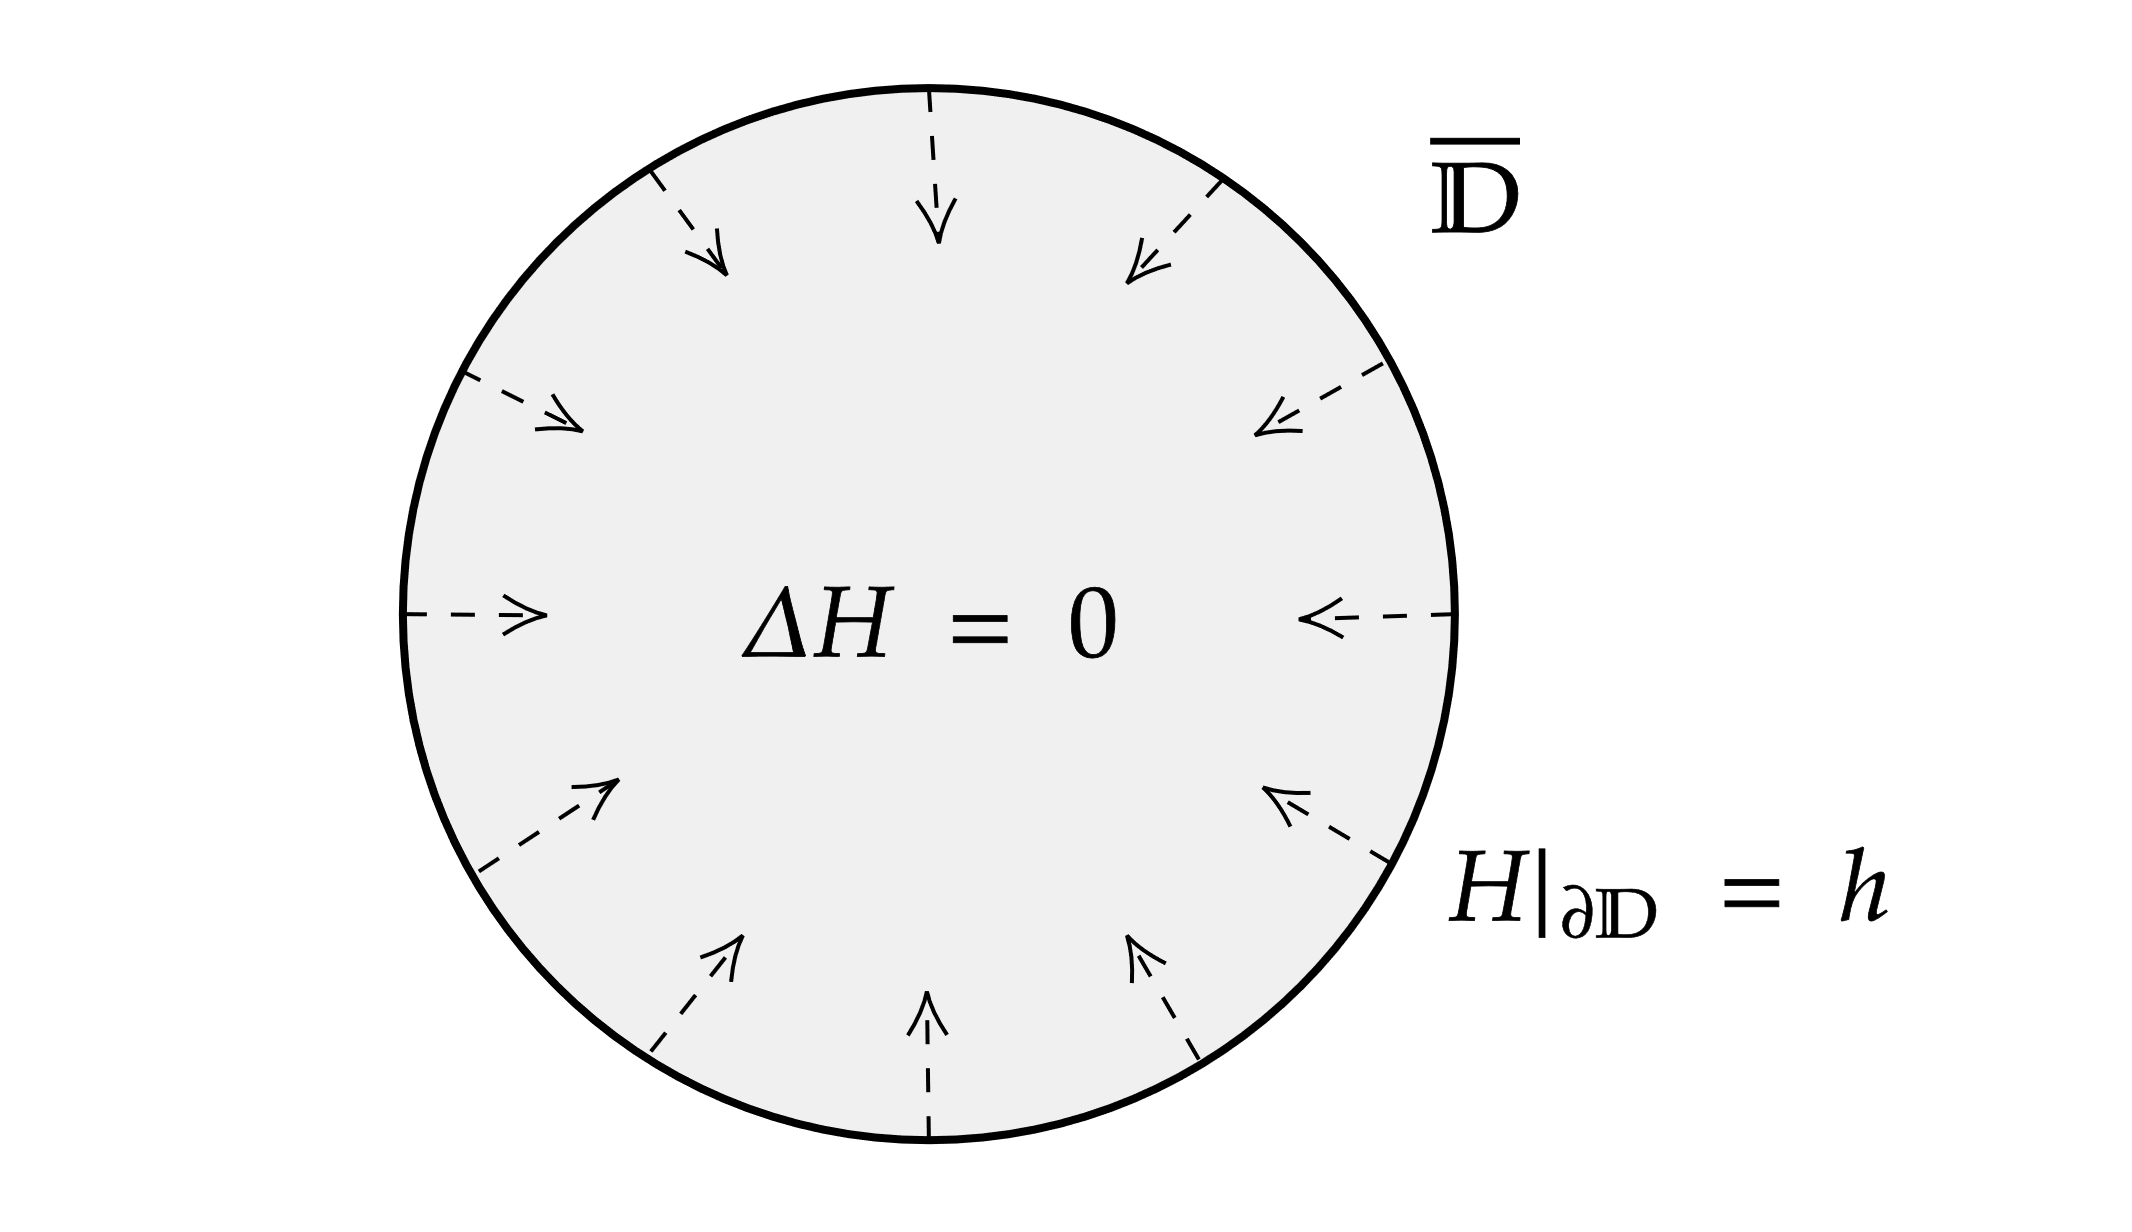
\includegraphics[width = \textwidth]{dirichlet_form.png}
            \caption{Dirichletov problem za enotski disk, z robnim pogojem $h$.}
        \end{center}    
    \end{figure}

    Kot smo že komentirali po definiciji \ref{harm}, so funkcije harmonične natanko tedaj ko zadoščajo Laplaceovi parcialni diferencialni enačbi.   
    Vredno je omeniti, da lahko na Dirichletov problem za enotski disk gledamo tudi iz stališča teorije diferencialnih enačb. Gre za problem iskanja funkcije, ki na notranjosti območja reši Laplaceovo diferencialno enačbo ob robnem pogoju, ki ga določa v naprej podana funkcija na robu območja.     
    V našem primeru je notranjost območja kar notranjost enotskega diska, robni pogoj zvezne funkcije pa podaja začetna zvezna funkcija, podana na enotski krožnici.
    Navadno se v teoriji parcialnih diferencialnih enačb srečamo s tako imenovanimi dobro postavljenimi matematičnimi problemi, o katerih si bralec več lahko prebere na REFERENCA.     
    V nadaljevanju se bomo le seznanili z njihovo definicijo in pokazali, da zgoraj zastavljen Dirichletov problem za enotski disk ustreza definiciji. 

    \begin{definicija}[J. Hadamard]
        \label{def_dp}
        Pravimo, da je matematičen problem parcialnih diferencialnih enačb z robnimi in začetnimi pogoji \emph{dobro postavljen}, če zanj velja
        \begin{enumerate}[label={\Alph*)}]
            \item rešitev problema obstaja,
            \item rešitev problema je enolično določena,
            \item rešitev je zvezno odvisna od začetnih podatkov problema.
        \end{enumerate}
    \end{definicija}

    \begin{lema}
        \label{enolicno}
        Če rešitev za Dirichletov problem na enotskem disku obstaja, je enolično določena.
    \end{lema}
    \begin{dokaz}
        Denimo, da obstajata dve različni rešitvi, $H_1$ in $H_2$, Dirichletovega problema za enotski disk z začetnim pogojem $h$.
        Oglejmo si razliko $H_1 - H_2$. Vemo, da je njuna razlika na $\partial \mathbb{D}$ enaka $0$, saj sta tam enaki $h$. 
        Ker sta funkciji $H_1$ in $H_2$ na $\mathbb{D}$ harmonični, je zaradi linearnosti Laplaceovega operatorja tudi njuna razlika harmonična funkcija. 
        Po posledici \ref{pm_harm}, oziroma principu maksima za harmonične funkcije sledi, da je $H_1 - H_2 \equiv 0$ tudi na $\mathbb{D}$. Sledi enakost $H_1$ in $H_2$ tudi na $\mathbb{D}$ in protislovje. 
    \end{dokaz}
    
    Lema \ref{enolicno} nam pove, da je rešitev problema največ ena. Zato se je dovolj posvetiti konstrukciji potencialne rešitve. 
    Opazimo, da lahko točke $z \in \partial \mathbb{D}$ zapišemo z \mbox{$e^{i \theta} \in \partial \mathbb{D}$}, kjer $\theta \in [0,2\pi]$. Funkcijo $h(z),~z \in \partial \mathbb{D}$ lahko tako pišemo kot kompozitum $h(e^{i \theta}),~\theta \in [0,2\pi]$.

    Sedaj poskusimo skonstruirati harmonično razširitev, ki bo zadoščala Dirichletovemu problemu na enotskem disku za zvezno funkcijo $h(e^{i \theta})$.
    Za začetek se posvetimo enostavnim primerom in si šele za tem teorijo oziroma konstrukcijo oglejmo v splošnem. 
    
    Naravno je za enostavne zvezne funkcije, definirane na $\partial \mathbb{D}$, vzeti kar polinome. Zgornji komentar nam pove, da je polinomska spremenljivka lahko kar $e^{i\theta}$, kjer \mbox{$\theta \in [0,2\pi]$}. 
    Zaradi linearnosti Laplaceovega operatorja se problem prevede na iskanje rešitve za monome. 
    Zato si oglejmo funkcije oblike $h(e^{i \theta}) = e^{i k \theta}, k \in \mathbb{Z}$, ter za njih poskusimo skonstruirati želeno razširitev. 
    Hitro opazimo, da se nam v tem primeru pojavlja preprosta eksplicitna razširitev s predpisom $H(r e^{i \theta}) = r^{|k|}e^{i k \theta}$, za \mbox{$r \in [0, 1]$} in $\theta \in [0, 2\pi]$. 
    Tako predpisana razširitev je za $k \geq 0$ na $\mathbb{D}$ harmonična, saj je $r^k e^{ik\theta} = z^k$ celo holomorfna funkcija in zato harmonična. Pri $k < 0$ dobimo razširitev $r^{-k} e^{ik\theta} = \overline{z}^{-k}$, ki v splošnem ni holomorfna, a je \mbox{kljub} temu harmonična. 
    Gre namreč za monom v konjugirani spremenljivki, harmoničnost katerega lahko preverimo po definiciji prek parcialnih odvodov.
    Obenem je za vsak $k \in \mathbb{Z}$ razširitev zvezna na $\overline{\mathbb{D}}$ in se na $\partial \mathbb{D}$ ujema z začetnimi pogoji. Razširitev torej zadošča pogojem za rešitev Dirichletovega problema na enotskem disku, ki je po lemi \ref{enolicno} enolično določena. 
    Ko upoštevamo linearnost Laplaceovega operatorja za začetne funkcije oblike $h(e^{i\theta}) = \sum_{k = -N}^{N}{a_k e^{ik\theta}},~\theta \in [0,2\pi]$ dobimo harmonično razširitev s predpisom
    $H(r e^{i \theta}) = \sum_{k = -N}^{N}{a_k r^{|k|}e^{ik\theta}},~r \in [0,1],~\theta \in [0,2\pi]$. 
    
    Smiselno bi bilo koeficiente $a_k$ izraziti direktno prek funkcije $h$. 
    V ta namen si oglejmo $\int_{-\pi}^{\pi}{e^{ij\theta} e^{-ik\theta}d\theta}$, kjer $k,l \in \mathbb{Z}$. Prek integracije zapisane kompleksne funkcije preverimo tako imenovano ortogonalno relacijo med kompleksnimi eksponenti
        $$
        \int_{-\pi}^{\pi}{e^{ij\theta} e^{-ik\theta}~\frac{d\theta}{2\pi}} = 
        \begin{cases}
            1~,~&j=k\\
            0~,~&j \neq k\\
        \end{cases}
        .$$
    Zgornja relacija nam pri $h(e^{i\theta}) = \sum_{k = -N}^{N}{a_k r^{|k|} e^{ik\theta}}$ omogoča izražavo koeficientov $a_k$ kot
        $$
            a_ k = \int_{-\pi}^{\pi}{h \left(e^{i\theta}\right)e^{-ik\theta}~\frac{d\theta}{2\pi}}.
        $$
    Z uporabo zgornje zveze izrazimo
    $$
        \sum_{k = - N}^{N}{ a_k r^{|k|}e^{ik\theta}} = \sum_{k = - N}^{N} \left(\int_{-\pi}^{\pi}{h(e^{i \varphi}) e^{- i k \varphi}~\frac{d \varphi}{2 \pi}}\right) r^{|k|} e^{i k \theta}.
    $$
    Zamenjamo vsoto in integral, ter množico, po kateri teče indeks vsote, razširimo na vsa cela števila. Pri tem se rezultat ne spremeni, saj je sumand pri dodanih indeksih enak nič. Dobimo ekspliciten zapis
    \begin{equation}
        \label{int1}
        \widetilde{h}(r e^{i \theta}) = \int_{-\pi}^{\pi}{h(e^{i \varphi}) \left(\sum_{k = - \infty}^{\infty} r^{|k|} e^{- i k \varphi} e^{i k \theta} \right) \frac{d \varphi}{2 \pi}}, ~~~ r e^{i\theta} \in \overline{\mathbb{D}}.
    \end{equation}
    Zgornji ekspliciten zapis razširitve je le drugače zapis že komentirane rešitve Dirichletovega problema na enotskem disku, za polinom v spremenljivki $e^{i \theta}$, \mbox{$\theta \in [0,2\pi]$}.
    
    Sedaj bomo zgornjo funkcijo, ki smo jo na intuitiven način konstruirali s pomočjo predpostavljene polinomske oblike funkcije $h$, vzeli za definicijo novega pojma in z njegovo pomočjo prišli do razširitve za splošne zvezne funkcije $h$.
    
\subsection{Poissonovo jedro}

    Osredotočimo se najprej na vrsto v integralu zapisa \eqref{int1}.

    \begin{definicija}
        \emph{Poissonovo jedro} je funkcija definirana s predpisom
        $$
           P_r(\theta) = \sum_{k = -\infty}^{\infty}{r^{|k|} e^{i k \theta}}\text{, kjer je}~\theta \in [-\pi, \pi]~\text{in}~ 0 < r < 1.
        $$
    \end{definicija}
    \begin{opomba}
        Na Poissonovo jedro lahko gledamo kot na funkcijo dveh spremenljivk, $\theta$ in $r$, ali pa kot na družino funkcij, indeksiranih s parametrom $r$.
    \end{opomba}

    Smiselno se je vprašati, ali za vsako vrednost iz definicijskega območje Poissonovega jedra vrsta na desni strani definicijske enakosti sploh konvergira. Potencialne strahove pomiri naslednja trditev.
    
    \begin{trditev}
        Naj bo $\rho < 1$. Vrsta, definirana s Poissonovim jedrom, konvergira enakomerno na množici $\{(r,\theta)~|~r \in [0,\rho],~ \theta \in [0,2\pi]\}$.
    \end{trditev}
    \begin{dokaz}
        Na množici $\{(r,\theta)~|~r \in [0,\rho],~ \theta \in [0,2\pi]\}$ velja $|r^{|k|} e^{i k \theta}| \leq \rho^{|k|}$. Ker je $\rho < 1$, številska vrsta $\sum_{k = -\infty}^{\infty}{\rho ^{|k|}}$ konvergira. 
        Po Weierstrassovem M-testu zato Poissonovo jedro konvergira enakomerno na množici $\{(r,\theta)~|~r \in [0,\rho],~ \theta \in [0,2\pi]\}$.
    \end{dokaz}

    Poissonovo jedro lahko zapišemo na več načinov. Če vrsto v definiciji Poissonovega jedra razbijemo na tri dele, glede na predznačenost indeksa vrste, za $z = r e^{i\theta} \in \mathbb{D}$ dobimo
    \begin{equation}
        \label{eq1}
        P_r(\theta) =  1 + \sum_{k = 1}^{\infty}{r^{k} e^{i k \theta}} +  \sum_{j = 1}^{\infty}{r^{j} e^{-i j \theta}}  = 1 + \sum_{k=1}^{\infty}{z^k} + \sum_{j=1}^{\infty}{\overline{z}^{j}}.
    \end{equation}
    Ker je Poissonovo jedro definirano na notranjosti enotskega diska, kjer je absolutna vrednost kompleksne spremenljivke manjša od ena, obe vrsti v zapisu \eqref{eq1} konvergirata.
    Ko ju seštejemo s formulo za geometrijsko vrsto dobimo
    \begin{equation}
        \label{eq2}
        P_r(\theta) = 1 + \frac{z}{1 - z}+ \frac{\overline{z}}{1 - \overline{z}} = \frac{1 - |z|^2}{|1-z|^2}~,~~~~z = r e^{i\theta} \in \mathbb{D}.
    \end{equation}
    Opazimo, da bi \eqref{eq2} lahko zapisali tudi nekoliko drugače. Velja
    \begin{align}
        \label{eq3}
        P_r(\theta) &= 1 + \frac{z}{1 - z}+ \frac{\overline{z}}{1 - \overline{z}} = 1 + \left(\frac{z}{1 - z} \right)+ \overline{\left(\frac{z}{1 - z}\right)} \notag \\
        &= 1 + 2~\text{Re}\left[\frac{z}{1-z}\right] =\text{Re}\left[\frac{1 + z}{1-z}\right], & &z = r e^{i\theta} \in \mathbb{D}.
    \end{align}
    Enakost $|1 - z|^2 = (\overline{1 - z})(1 - z) = (1 - \overline{z})(1 - z) = 1 + r^2 - 2r \cos\theta$ pa nam omogoči zapis
    \begin{equation}
        \label{eq4}
        P_r(\theta) = \frac{1-r^2}{1+ r^2 - 2r \cos\theta}~,~~~~r \in [0,1),~\theta \in [0,2\pi].
    \end{equation}

    Preden se lotimo uporabe Poissonovega jedra, si s pomočjo zgornjih zapisov oglejmo še nekaj njegovih lastnosti, ki so zbrane v spodnjih trditvah. 
    
    \begin{trditev}
        \label{lastpk}
        Poissonovo jedro ima naslednje lastnosti:
        \begin{enumerate}[label={\alph*)}]
            \item kot funkcija spremenljivke $\theta$ je periodično s periodo $2\pi$, 
            \item za vsak $r \in [0,1)~\text{in vsak}~\theta \in [0,2\pi]~\text{je}~P_r(-\theta) = P_r(\theta)$,
            \item za vsak $r \in [0,1)~\text{funkcija}~P_r(\theta)~\text{za}~\theta \in [-\pi, 0 ]~\text{narašča in za}~\theta \in [0, \pi ]~\text{pada}$,
            \item za vsak $r \in [0,1)~\text{in vsak}~\theta\in [0,2\pi]~\text{je}~P_r(\theta) > 0$,
            \item za vsak $r \in [0,1)~\text{velja}~\int_{-\pi}^{\pi}{P_r(\theta) \frac{d\theta}{2\pi}} = 1$.
        \end{enumerate}
    \end{trditev}
    \begin{dokaz}
        Lastnosti a), b) in c) sledijo iz zapisa \eqref{eq4}. Opazimo, da je v tem zapisu od $\theta$ odvisen le člen s funkcijo kosinus. 
        Ta zagotavlja $2\pi$-periodičnost in sodost, ter podaja želen interval naraščanja in padanja Poissonovega jedra v odvisnosti od spremenljivke $\theta$. 
        
        Za dokaz točke d) si oglejmo zapis \eqref{eq2}. Ker je Poissonovo jedro definirano na notranjosti enotskega diska, je absolutna vrednost v zapisu uporabljene kompleksne spremenljive manjša od ena. 
        Sledi, da sta števec in imenovalec v zapisu strogo pozitivna, kar dokazuje trditev. 

        Pri dokazu točke e), si pomagajmo z izpeljavo rešitve za Dirichletov problem na enotskem disku. 
        Za robni pogoj, bomo na robu enotskega diska vzeli funkcijo, ki je identično enaka $1$. Označimo torej $h(z) \equiv 1,~ z \in \partial \mathbb{D}$. Opazimo, da je \mbox{$H(z) \equiv 1,~z \in \overline{\mathbb{D}}$} trivialna rešitev tako postavljenega Dirichletovega problema za enotski disk.
        Lema \ref{enolicno} nam pove, da je rešitev za tako podan Dirichletov problem enolično določena. Vemo tudi, da je harmonična razširitev eksplicitno podana prek formule \eqref{int1}.
        Velja torej
        $$
        1 = \int_{-\pi}^{\pi}{\left(\sum_{k=-\infty}^{\infty}{r^{|k|} e^{ik(\theta - \varphi)}}\right) \frac{d \varphi}{2 \pi}} = \int_{-\pi}^{\pi}{P_r(\theta - \varphi)\frac{d \varphi}{2 \pi}}~. 
        $$
        Sedaj v integral uvedemo novo spremenljivko $\tau = \theta - \varphi$. Zaradi periodičnosti Poissonovega jedra velja 
        $$
        1 = \int_{\theta - \pi}^{\theta + \pi}{P_r(\tau)~\frac{d \tau}{2 \pi}} = \int_{-\pi}^{\pi}{P_r(\tau)~\frac{d \tau}{2 \pi}}.
        $$
    \end{dokaz}

    \begin{posledica}
        Za vsak $r \in [0, 1)$ funkcija $\frac{1}{2 \pi} P_r(\theta),~ \theta \in [-\pi, \pi]$ določa gostoto zvezno porazdeljene slučajne spremenljivke.
    \end{posledica}
    \begin{dokaz}
        Iz zapisa \eqref{eq4} je jasno, da je pri poljubnem $r \in [0,1)$ zapisana funkcija v odvisnosti od $\theta$ zvezna na intervalu $[-\pi, \pi]$, točki d) in e) trditve \ref{lastpk} pa nam dokazujeta, da je na definicijskem območju funkcija strogo pozitivna in se pointegrira v $1$.
    \end{dokaz}

    \begin{trditev}
        \label{proti0}
        Naj bo $\delta > 0$. Potem gre $\max\{P_r(\theta)~|~ \delta \leq |\theta| \leq \pi\} \to 0$ ko gre $r \to 1$.
    \end{trditev}
    \begin{dokaz}
        Ker je za vsak $r$ Poissonovo jedro v odvisnosti od spremenljivke $\theta$ na intervalu $[-\pi, \pi]$ zvezna funkcija, maksimum na kompaktu $[-\pi, \pi]$ gotovo zavzamemo. Točki a) in b) trditve \ref{lastpk} nam povesta, da bomo za vsak $r$ maksimum zavzeli kar v $\delta$. 
        Oglejmo si torej $P_r(\delta) = \frac{1 -r^2}{1 + r^2 - 2r \cos\delta}$. Ker je $\delta >0 $, bo imenovalec ulomka strogo pozitiven, števec ulomka pa gre proti $0$, ko gre $r \to 1$. 
        Sledi, da gre \mbox{$\max\{P_r(\theta)~|~ \delta \leq |\theta| \leq \pi\} = P_r(\delta) \to 0$}, ko gre $r \to 1$.
    \end{dokaz}
    \begin{posledica}
        \label{int_proti0}
        Naj bo $\delta > 0$. Potem gre ${\int_{\{\pi \geq |\theta| \geq \delta\}}{P_{r}(\theta)~\frac{d\theta}{2 \pi}}} \to 0$, ko gre $r \to 1$.
    \end{posledica}
    \begin{dokaz}
        Ker je interval po katerem integriramo zaprt, Poissonovo jedro pa v odvisnosti od spremenljivke $\theta$ zvezna funkcija, za vsak $r \in [0,1)$ obstaja $c_r \in \mathbb{R}$, da velja $c_r = \max\{P_r(\theta)~|~ \delta \leq |\theta| \leq \pi\}$. Zato velja
        $$
        {\int_{\{\pi \geq |\theta| \geq \delta\}}{P_{r}(\theta)~\frac{d\theta}{2 \pi}}} \leq {\int_{\{\pi \geq |\theta| \geq \delta\}}{c_r~\frac{d\theta}{2 \pi}}} \leq c_r.
        $$
        Sedaj uporabimo trditev \ref{proti0}, ki nam pove, da gre $c_r \to 0$, ko gre $r \to 1$. Sledi, da gre tudi zapisan integral proti $0$, ko gre $r \to 1$.
    \end{dokaz}

    Oglejmo si lastnosti družine $\left\{ \frac{1}{2 \pi} P_r~|~r \in [0,1)\right\}$. Trditev \ref{lastpk} nam pove, da za vsak $r \in [0,1)$ velja $\frac{1}{2\pi}\int_{\partial \mathbb{D}}{P_r(\theta)} = 1$ in $P_r(\theta) > 0$ za vsak $\theta \in [0, 2 \pi]$.
    Zato velja tudi sup$\left\{\frac{1}{2 \pi}\int_{\partial \mathbb{D}}{\left| P_{r}\right|}~|~r \in [0,1)\right\}= 1$. Družino funkcij, ki obenem zadošča tudi lastnosti iz posledice \ref{int_proti0} imenujeno približna enota. 
    Bralec si več lahko prebere na REFERENCA.
 
    Vredno je, s pomočjo zgoraj zapisanih trditev, komentirati tudi obnašanje funkcije Poissonovega jedra, ko pošljemo $r \to 1$. Trditev \ref{proti0} nam pove, da se vrednosti funkcije, v odvisnosti od spremenljivke $\theta$, ki so poljubno malo oddaljene od izhodišča, približujejo $0$. 
    Zapisano dodatno potrdi tudi posledica \ref{int_proti0}.
    Oglejmo si sedaj, kaj se zgodi z vrednostjo funkcije pri $\theta = 0$, ko pošljemo $r \to 1$. Iz zapisa \eqref{eq4} vemo, da velja
    $$
    P_r(0) = \frac{1-r^2}{1+ r^2 - 2r} = \frac{1- r^2}{(1 - r)^2} = \frac{1 + r}{1 -r},~~r \in [0,1).
    $$
    Ko gre $r \to 1$, gre torej $P_r(0) \to \infty$. Zapisani opažanji nam skupaj z ugotovitvijo iz točke e) trditve \ref{lastpk} nakazujeta, da se Poissonovo jedro, ko pošljemo $r \to 1$, približuje tako imenovani Diracovi delti. 
    O tem si bralec več lahko prebere na REFERENCA.

    Navedene lastnosti Poissonovega jedra so tudi dobro razvidne na spodnji sliki. 

    \begin{figure}[H]
        \begin{center}
        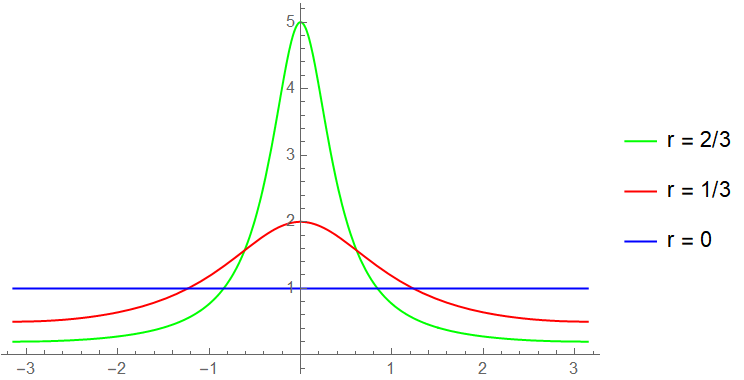
\includegraphics[width=\linewidth]{grafi.png}
        \caption{Graf Poissonovega jedra glede na vrednost spremenljivke $r$.}
        \end{center}    
    \end{figure}

    \begin{trditev}
        \label{poiss_harm}
        Poissonovo jedro je na enotskem disku harmonična funkcija. 
    \end{trditev}
    \begin{dokaz}
        Trditev \ref{hh} nam pove, da je dovolj pokazati, da lahko Poissonovo jedro zapišemo kot realni del holomorfne funkcije, definirane na enotskem disku.
        Zapis \eqref{eq3} nam pove, da je Poissonovo jedro realni del funkcije $f(z) = \frac{1 + z}{1 - z},~z \in \mathbb{D}$. Ker je $f$ na enotskem disku tudi holomorfna, je trditev s tem dokazana. 
    \end{dokaz}

    Ker je enotski disk zvezdasto območje, Poissonovo jedro pa po trditvi \ref{poiss_harm} harmonična funkcija, po trditvi \ref{konj} obstaja harmonična konjugiranka Poissonovega jedra. 
    Opazimo, da smo v zapisu \eqref{eq3} Poissonovo jedro prikladno zapisali kot realni del holomorfne funkcije, zato se nam ponuja harmonična konjugiranka Poissonovega jedra kot imaginarni del zapisane holomorfne funkcije.
    Velja
    \begin{align*}
        \text{Im}\left[\frac{1 + z}{1-z}\right] &= \frac{\frac{1 + z}{1-z} - \left(\overline{\frac{1 + z}{1-z}}\right)}{2i} = \frac{(1 + z)(1 - \overline{z}) - (1 + \overline{z})(1 - z)}{|1 - z|^2~2i} & & \\ 
        & = \frac{2 (z - \overline{z})}{|1 - z|^2~2i} = \frac{2~\text{Im}z}{|1 - z|^2} = \frac{2 r \sin\theta}{1+ r^2 - 2r \cos\theta}~, & & z = r e^{i\theta} \in \mathbb{D}.
    \end{align*}
    Prav to je motivacija za naslednjo definicijo. 
    \begin{definicija}
        \emph{Konjugirano Poissonovo jedro} je funkcija definirana s predpisom
        \begin{align}
            Q_r(\theta) & = \frac{2 r \sin\theta}{1+ r^2 - 2r \cos\theta}~,~~r \in [0,1),~\theta \in [0,2\pi].
        \end{align}
    \end{definicija}

    Zapišimo zvezi, ki jih narekujeta zgornji komentar in definicija. Velja
    $$
    P_r(\theta) + i~Q_r(\theta) = \left( \frac{1-r^2}{1+ r^2 - 2r \cos\theta}\right) + i \left(\frac{2 r \sin\theta}{1+ r^2 - 2r \cos\theta}\right) = \frac{1 + re^{i\theta}}{1 - re^{i\theta}}~,~~r e^{i\theta} \in \mathbb{D}.
    $$      

    Sedaj se vrnimo k reševanju Dirichletovega problema za enotski disk. 
    Spomnimo se, da smo za polinomske funkcije $h$ skonstruirali predpis razširitve, ki je rešila zastavljen problem. 
    Opazimo, da bi si pri zapisu enačbe \eqref{int1} lahko pomagali z definiranim pojmom Poissonovega jedra. Zapišemo lahko
    $$
    H(r e^{i \theta}) = \int_{-\pi}^{\pi}{h(e^{i \varphi}) \left(\sum_{k = - \infty}^{\infty} r^{|k|} e^{- i k \varphi} e^{i k \theta} \right)}\frac{d \varphi}{2 \pi} = 
    \int_{-\pi}^{\pi}{h(e^{i \varphi}) P_r(\theta - \varphi)\frac{d \varphi}{2 \pi}},~~r e^{i \theta} \in \overline{\mathbb{D}}.
    $$

    Zgoraj smo z intuitivno izpeljavo nevede že zapisali funkcijo, ki jo bomo sedaj vzeli za definicijo novega pojma. 
    Pokazali bomo, da to tudi pri splošnih zveznih funkcijah omogoča zapis rešitve Dirichletovega problema na enotskem disku.

\subsection{Poissonov integral}

    Tako kot smo to storili v prejšnem razdelku, začnimo z definicijo novega pojma.

    \begin{definicija}
        Naj bo $h(e^{i \theta})$ zvezna funkcija, definirana na robu enotskega diska.
        \emph{Poissonov integral} funkcije $h(e^{i\theta})$, ki ga označimo s $\widetilde{h}(z)$, je funkcija, definirana na notranjosti enotskega diska s predpisom
        $$
        \widetilde{h}(z) = \int_{0}^{2\pi}{h(e^{i\varphi}) P_r(\theta - \varphi)~\frac{d\varphi}{2 \pi}}~,~~z = r e^{i\theta} \in \mathbb{D}.
        $$
     \end{definicija}
     \begin{opomba}
        \label{kom_poiss}
        Če v zgornji integral uvedemo novo spremenljivko $\tau = \theta - \varphi$, ter upoštevamo periodičnost Poissonovega jedra, lahko Poissonov integral funkcije $h$, zapišemo tudi kot
        $$
        \widetilde{h}(z) = \int_{0}^{2\pi}{h\big(e^{i(\theta-\varphi)}\big) P_r(\varphi)~\frac{d\varphi}{2 \pi}}~,~~z = r e^{i\theta} \in \mathbb{D}.
        $$
        Natančneje si opisan postopek, ki pripelje do zgornjega zapisa Poissonovega integrala bralec lahko ogleda v dokazu točke e) trditve \ref{lastpk}.
     \end{opomba}

    Oglejmo si še nekoliko drugačen zapis Poissonovega integrala za zvezno funkcijo $h(e^{i \theta})$.
    Če definiramo funkcijo $f(w) = h(e^{iw})$, lahko Poissonov integral zapišemo kot
    \begin{align}
        \label{konv_Pr}
        \widetilde{h}(z) &= \int_{0}^{2\pi}{h(e^{i\varphi}) P_r(\theta - \varphi)~\frac{d\varphi}{2 \pi}} = \int_{0}^{2\pi}{f(\varphi) P_r(\theta - \varphi)~\frac{d\varphi}{2 \pi}} \notag \\
        & = \frac{1}{2\pi} \left[(f * P_r)(\theta)\right] = \frac{1}{2\pi} \left[(P_r * f)(\theta)\right],~~z = r e^{i\theta},~\theta \in [0,2\pi],~r\in[0,1).
    \end{align}
    \begin{opomba}
        Zadnja enakost v zgornjem zapisu je posledica komutativnosti konvolucije ter še na nekoliko drugačen način dokazuje zapis iz opombe \ref{kom_poiss}. Velja namreč
        \begin{align*}
            \widetilde{h}\left(r e^{i \theta}\right) &= \frac{1}{2\pi} \left[(P_r * f)(\theta)\right] =  \frac{1}{2 \pi}\int_{0}^{2\pi}{P_r(\varphi) f(\theta - \varphi) ~d\varphi} \\
            & = \int_{0}^{2\pi}{h\big(e^{i(\theta-\varphi)}\big) P_r(\varphi)~\frac{d\varphi}{2 \pi}},~~z = r e^{i\theta},~\theta \in [0,2\pi],~r\in[0,1). \notag
        \end{align*}
    \end{opomba}

    Ogledali smo si alternativni zapis Poissonovega integrala s konvolucijo Poissonovega jedra. Smiselno se je vprašati, kako na zgornji postopek zapisa s konvolucijo vpliva zamenjava Poissonovega jedra s konjugiranim Poissonovim jedrom. Opazimo, da lahko po enakem postopku tudi integral s konjugiranim Poissonovim jedrom izrazimo kot konvolucijo. 
    Ponovno definiramo $f(w) = h(e^{i w})$, ki nam omogoča zapis
    \begin{align}
        \label{konv_Qr}
        \int_{0}^{2\pi}{h(e^{i\varphi}) Q_r(\theta - \varphi)~\frac{d\varphi}{2 \pi}}  &= \frac{1}{2\pi}\int_{0}^{2 \pi}{f(\varphi) Q_r(\theta - \varphi)~d\varphi} \\ 
        &= \frac{1}{2 \pi}[(f * Q_r)(\theta)]~,~~z = r e^{i\theta},~\theta \in [0,2\pi],~r\in[0,1). \notag
    \end{align}
    
    Konvolucijska zapisa integrala bomo uporabili nekoliko kasneje, sedaj pa se še nekoliko posvetimo lastnostim Poissonovega integrala.

    \begin{trditev}
       \label{lastpi}
       Naj bo $\Phi$ preslikava, ki zvezni funkciji $h$, definirani na robu enotskega diska, prireredi njen Poissonov integral $\widetilde{h}$, tj. $\Phi : h \mapsto \widetilde{h}$.
       Potem velja
       \begin{enumerate}[label={\alph*)}]
           \item $\Phi$ je kompleksno linearna preslikava, tj. $\text{za vsak}~h_1,h_2 \in C^0(\partial \mathbb{D})$ in vsak $c_1,c_2 \in \mathbb{C}$ velja $\Phi(c_1 h_1 + c_2 h_2) = c_1 \Phi(h_1) + c_2 \Phi(h_2)$,
           \item $\Phi$ ohranja omejenost, tj. če za $h \in C^0(\partial \mathbb{D})$ in $M \in \mathbb{R}$ velja $|h(z)| \leq M$, za vsak $z \in \partial \mathbb{D}$, potem je $|[\Phi(h)](z)| \leq M$ za vsak $z \in \mathbb{D}$.
       \end{enumerate}
    \end{trditev}
    \begin{dokaz}
           Dokažimo najprej točko a). Naj bosta $h_1$ in $h_2$ poljubni zvezni funkciji, definirani na robu enotskega diska, ter $c_1, c_2$ poljubni kompleksni števili. 
           Potem je na robu enotskega diska zvezna tudi funkcija $c_1 h_1 + c_2 h_2$. Oglejmo si sedaj najprej Poissonov integral za zapisano linearno kombinacijo. Velja
           \begin{align*}
               [\widetilde{c_1 h_1 + c_2 h_2}](z) &= \int_{-\pi}^{\pi}{\left([c_1 h_1 + c_2 h_2](e^{i\varphi}) \right)P_r(\theta - \varphi)~\frac{d\varphi}{2 \pi}}\\ 
               & = \int_{-\pi}^{\pi}{\left([c_1 h_1](e^{i\varphi}) + [c_2 h_2](e^{i\varphi})\right)P_r(\theta - \varphi)~\frac{d\varphi}{2 \pi}}\\
               & = c_1\int_{-\pi}^{\pi}{h_1(e^{i\varphi})P_r(\theta - \varphi)~\frac{d\varphi}{2 \pi}} + c_2\int_{-\pi}^{\pi}{h_2(e^{i\varphi})P_r(\theta - \varphi)~\frac{d\varphi}{2 \pi}}\\
               & = c_1 \widetilde{h_1}(z) + c_2 \widetilde{h_2}(z) = [c_1 \widetilde{h_1} + c_2 \widetilde{h_2}](z)~,~~~z \in \mathbb{D}.
           \end{align*}
           Po definiciji preslikave $\Phi$ sedaj sledi $\Phi(c_1 h_1 + c_2 h_2) = c_1 \Phi(h_1) + c_2 \Phi(h_2)$.
           
           Dokažimo še točko b). Naj bo $h$ poljubna omejena zvezna funkcija, definirana na robu enotskega diska. Naj za $M \in \mathbb{R}$ velja $|h(z)| \leq M$, za vsak $z \in \partial \mathbb{D}$.
           Ponovno si najprej oglejmo Poissonov integral funkcije $h$ in uporabimo zapisano neenakost, ter točki d) in e) trditve \ref{lastpk}. Dobimo
           \begin{align*}
               \left|\widetilde{h}(z)\right| &= \left| \int_{-\pi}^{\pi}{h(e^{i\varphi}) P_r(\theta - \varphi)~\frac{d\varphi}{2 \pi}} \right| \leq \int_{-\pi}^{\pi}{\left|h(e^{i\varphi}) \right|P_r(\theta - \varphi)~\frac{d\varphi}{2 \pi}} \\ 
               &\leq M \int_{-\pi}^{\pi}{P_r(\theta - \varphi)~\frac{d\varphi}{2 \pi}} = M~,~~~z \in \mathbb{D}.& & \\
           \end{align*}
           Po definiciji preslikave $\Phi$ zato $|[\Phi(h)](z)| \leq M$, za vsak $z \in \mathbb{D}$.
    \end{dokaz}

\subsection{Schwarzova integralska formula}

    Za trenutek se oddaljimo od reševanja Dirichletovega problema, ter vpeljane pojme uporabimo za dokaz Schwarzove integralske formule.

     \begin{lema}
        \label{realnidel}
        Naj bo $u$ realna zvezna funkcija, definirana na $\partial \mathbb{D}$. Potem je Poissonov integral funkcije $u$ na $\mathbb{D}$ harmonična funkcija.
     \end{lema}
     \begin{dokaz}
        Pomagajmo si z zapisom \eqref{eq3}. Za $z = re^{i\theta} \in \mathbb{D}$ lahko zapišemo
            \begin{align}
                \label{lema_schwarz}
                \widetilde{u}(z) &= \widetilde{u}(r e^{i \theta}) = \int_{-\pi}^{\pi}{u(e^{i \varphi}) P_r(\theta - \varphi)\frac{d \varphi}{2 \pi}} = \int_{-\pi}^{\pi}{u(e^{i \varphi})~\text{Re}\left[\frac{1+re^{i(\theta - \varphi)}}{1-re^{i(\theta - \varphi)}}\right]\frac{d \varphi}{2 \pi}} \notag \\
                &= \int_{-\pi}^{\pi}{u(e^{i \varphi})~\text{Re}\left[\frac{e^{i\varphi}+re^{i\theta}}{e^{i\varphi}-re^{i\theta}}\right]\frac{d \varphi}{2 \pi}}=~\text{Re}\left[\int_{-\pi}^{\pi}{u(e^{i \varphi})\bigg(\frac{e^{i\varphi}+z}{e^{i\varphi}-z}\bigg)\frac{d \varphi}{2 \pi}}\right].
            \end{align}
        Tako smo $\widetilde{u}(z)$ za $z \in \mathbb{D}$ izrazili kot realni del holomorfne funkcije, kar po trditvi \ref{hh} dokazuje harmoničnost Poissonovega integrala funkcije $u$, na notranjosti enotskega diska.
     \end{dokaz}

     Osredotočimo se na predpis holomorfne funkcije iz zapisa \eqref{lema_schwarz}. Opazimo, da smo jo konstruirali s pomočjo podane realne funkcije $u$. 
     Sedaj začnimo nekoliko drugače. Denimo da imamo podano funkcijo $F = U + iV$, ki je na $\overline{\mathbb{D}}$ zvezna in na $\mathbb{D}$ holomorfna. Vredno je omeniti, da sta tu v zapisu $U$ in $V$ realni funkciji, ki predstavljata realni oziroma imaginarni del funkcije $F$, ter sta zato na $\overline{\mathbb{D}}$ zvezni in na $\mathbb{D}$ harmonični.
     Iz realnega dela holomorfne funkcije $F$, torej funkcije $U$, lahko na enak način kot smo to storili v \eqref{lema_schwarz}, konstruiramo holomorfno funkcijo $\widetilde{F}$ s predpisom
     \begin{equation}
        \label{priprav_schwarz}
        \widetilde{F}(z) = \int_{0}^{2 \pi}{U(e^{i \varphi})\bigg(\frac{e^{i\varphi}+z}{e^{i\varphi}-z}\bigg)\frac{d \varphi}{2 \pi}}~,~~z \in \mathbb{D}.
    \end{equation}
    Enakost \eqref{lema_schwarz} nam pove, da za $z = r e^{i\theta}\in \mathbb{D}$ velja $\text{Re}[\widetilde{F}(z)] = U(z)$. Smiselno se je vprašati ali lahko kaj podobnega na $\mathbb{D}$ trdimo tudi za $\widetilde{F}$ in $F$. 
    O tem nam več pove naslednja trditev. 

    \begin{trditev}[Schwarzova integralska formula]
        \label{schwarz_int_f}
        Naj bo $F = U + iV$ funkcija, holomorfna na $\mathbb{D}$ in zvezna na $\overline{\mathbb{D}}$. Potem velja
        $$ 
            F(z) = \int_{0}^{2 \pi}{U(e^{i \varphi})\bigg(\frac{e^{i\varphi}+z}{e^{i\varphi}-z}\bigg)\frac{d \varphi}{2 \pi}} + i V(0)~,~~z \in \mathbb{D}.
        $$
    \end{trditev}
    \begin{dokaz}
        Enako kot smo to storili v \eqref{lema_schwarz} in \eqref{priprav_schwarz}, lahko definiramo holomorfno funkcijo
        $$
        \widetilde{F}(z) = \int_{0}^{2 \pi}{U(e^{i \varphi})\bigg(\frac{e^{i\varphi}+z}{e^{i\varphi}-z}\bigg)\frac{d \varphi}{2 \pi}},~z \in \mathbb{D}.
        $$
        Komentirali smo že, da po \eqref{lema_schwarz} velja $\text{Re}[\widetilde{F}] \equiv \text{Re}[F]$, oziroma $\text{Re}[(\widetilde{F} - F)(z)] = 0$, za vsak $z \in \mathbb{D}$. 
        Razlika holomorfnih funkcij zadošča Cauchy-Riemannovemu sistemu enačb, zato obstaja $C \in \mathbb{C}$, da velja $\text{Im}[(\widetilde{F} - F)(z)] = C$ za vsak $z \in \mathbb{D}$.
        Ker je $U$ na $\mathbb{D}$ harmonična, ima na $\mathbb{D}$ lastnost povprečne vrednosti. Zato velja
        $$
        \widetilde{F}(0) = \int_{0}^{2 \pi}{U(e^{i \varphi})\bigg(\frac{e^{i\varphi}+0}{e^{i\varphi}-0}\bigg)\frac{d \varphi}{2 \pi}} = \int_{0}^{2 \pi}{U(e^{i \varphi})\frac{d \varphi}{2 \pi}} = U(0).
        $$
        Ker je $F(0) = U(0) + iV(0)$, sledi $\text{Im}[F - \widetilde{F}] \equiv V(0)$.
        Torej velja
        $$ 
        F(z) = \widetilde{F}(z) + iV(0) = \int_{0}^{2 \pi}{U(e^{i \varphi})\bigg(\frac{e^{i\varphi}+z}{e^{i\varphi}-z}\bigg)\frac{d \varphi}{2 \pi}} + i V(0)~,~~z \in \mathbb{D}.
        $$
    \end{dokaz}

    Spomnimo se zapisov \eqref{konv_Pr} in \eqref{konv_Qr}. Schwarzovo integralsko formulo iz trditve \ref{schwarz_int_f}, lahko za holomorfno funkcijo $F = U + iV$ alternativno zapišemo kot konvolucijo. Velja
    $$
        F(r e^{i \theta}) = \int_{0}^{2 \pi}{U(e^{i \varphi})\left(\frac{e^{i \varphi}+r e^{i \theta}}{e^{i \varphi}-r e^{i \theta}}\right)\frac{d \varphi}{2 \pi}} + i V(0)~,~~\theta \in [0,2 \pi],~r \in [0,1).
    $$
    Sedaj označimo $G(w) = U(e^{iw})$, ter poenostavimo. Dobimo
    \begin{align*}
        F(r e^{i \theta}) & = \int_{0}^{2 \pi}{G(\varphi)\left(\frac{1 +r e^{i (\theta-\varphi)}}{1-r e^{i(\theta-\varphi)}}\right)}\frac{d\varphi}{2 \pi} + iV(0)\\
        & = \frac{1}{2 \pi} \left(\int_{0}^{2 \pi}{G(\varphi)[(P_r + i Q_r)(\theta - \varphi)]}~d\varphi\right)+  iV(0) \\
        & = \frac{1}{2 \pi} \left[G * (P_r + iQ_r)\right](\theta) + iV(0)\\
        & = \frac{1}{2 \pi}\left((G * P_r)(t) + i\big[(G * Q_r)(t) + 2 \pi V(0)\big]\right),~~\theta\in [0,2 \pi],~r \in [0,1).
    \end{align*}

\subsection{Rešitev Dirichletovega problema na enotskem disku}
    Vrnimo se k bistvu razdelka. Za preproste zvezne funkcije smo že dokazali, da rešitev Dirichletovega problema na enotskem disku obstaja. To nas je pripeljalo do definicije Poissonovega jedra in Poissonovega integrala, s pomočjo katerih bomo sedaj pokazali, da za poljubno zvezno funkcijo obstaja rešitev Dirichletovega problema na enotskem disku.
    \begin{trditev}
        \label{obstoj}
        Naj bo $h$ zvezna kompleksna funkcija, definirana na $\partial \mathbb{D}$. Rešitev Dirichletovega problema, z robnim pogojem $h$, za enotski disk obstaja in je na $\mathbb{D}$ definirana kot Poissonov integral funkcije $h$.
    \end{trditev}
    \begin{opomba}
        \label{opomba_obstoj}
        Definirajmo funkcijo $H$, na $\overline{\mathbb{D}}$, kot
        $$
            H(z) = \begin{cases}
                    h(z),~~z \in \partial \mathbb{D}\\
                    \widetilde{h}(z),~~z \in \mathbb{D}
            \end{cases},~~~~\text{kjer je}~\widetilde{h}~\text{Poissonov integral funkcije}~h.
        $$
        Zgornja trditev pravi, da je funkcija $H$ rešitev Dirichletovega problema za enotski disk z robnim pogojem $h$. 
        %
        %na $\overline{\mathbb{D}}$ zvezna, ter na $\mathbb{D}$ harmonična. Po definiciji funkcije $H$ opazimo, da bo potrebno da je na $\mathbb{D}$ harmoničen Poissonov integral funkcije $h$. 
        %Ker se zožitev tako definirane funkcije $H$ na $\partial \mathbb{D}$ ujema s $h$, želimo dokazati, da je ravno funkcija $H$ rešitev za Dirichletov problem na enotskem disku, z robnim pogojem $h$. 
        %
        Formulacijo problema smo predstavili tudi grafično, pa naredimo to še za rešitev problema. 
        \begin{figure}[H]
            \begin{center}
                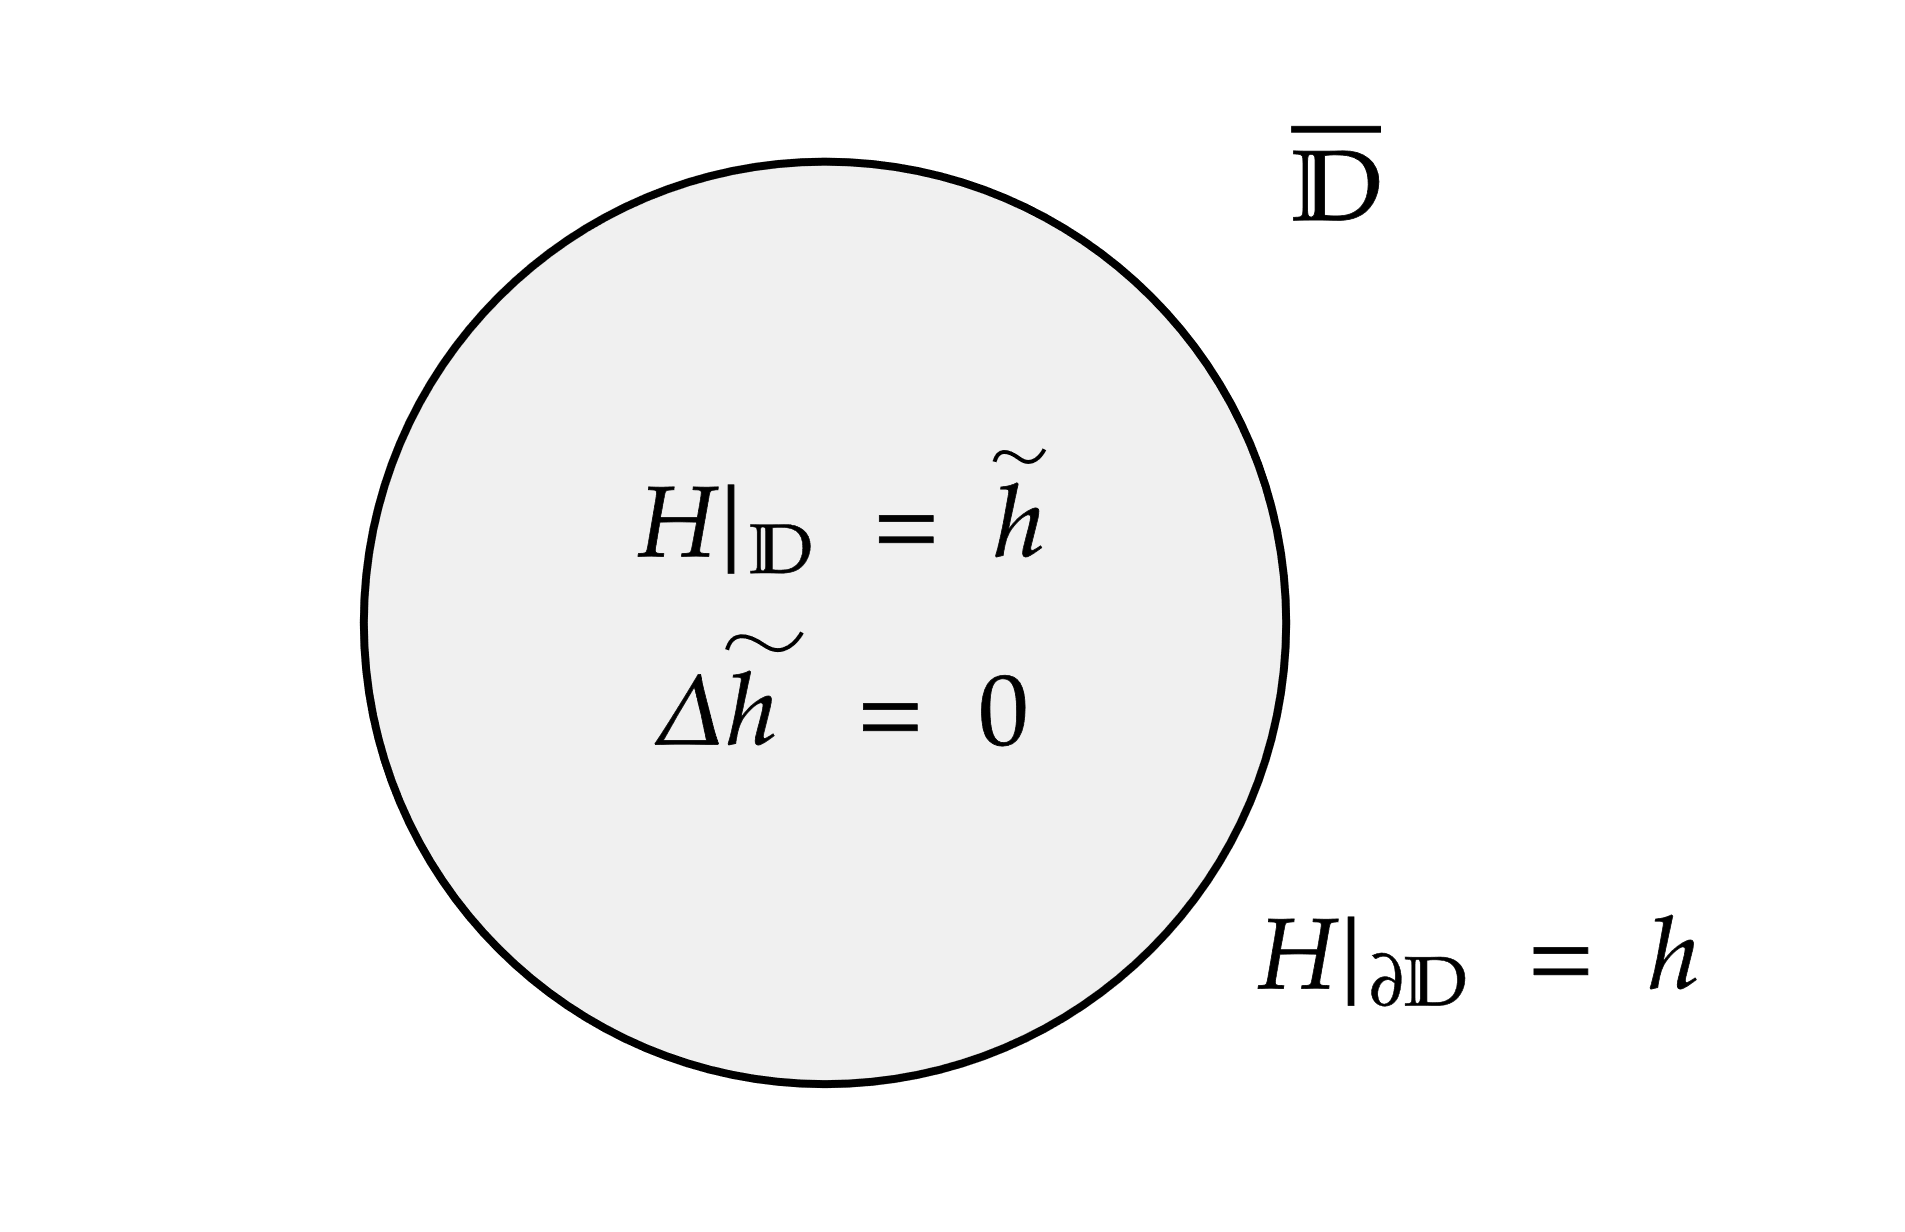
\includegraphics[width = \textwidth]{dirichlet_resitev.png}
                \caption{Rešitev Dirichletovega problema na enotskem disku, z robnim pogojem $h$.}
            \end{center}    
        \end{figure}
     \end{opomba}

     \begin{dokaz}
        Trditev bomo dokazali v dveh korakih. Najprej dokažimo, da je Poissonov integral na $\mathbb{D}$ harmonična funkcija.
        Vemo, da lahko kompleksno funkcijo $h$ razcepimo na njen realni in imaginarni del kot $h = u + iv$, kjer sta $u$ in $v$ realni funkciji. 
        Točka a) trditve \ref{lastpi} nam pove, da velja $\widetilde{h} = \widetilde{u} + i \widetilde{v}$.
        Ker sta $u$ in $v$ realni zvezni funkciji, definirani na robu enotskega diska, lahko uporabimo lemo \ref{realnidel}. Ta nam pove, da sta $\widetilde{u}$ in $\widetilde{v}$ na $\mathbb{D}$ harmonični funkciji. 
        Iz linearnosti Laplaceovega operatorja sledi, da je potem tudi $\widetilde{h} = \widetilde{u} + i \widetilde{v}$ na $\mathbb{D}$ harmonična funkcija.
        
        Za dokaz zveznosti na $\overline{\mathbb{D}}$ se moramo nekoliko bolj potruditi. Tako kot smo to storili v opombi \ref{opomba_obstoj}, s $H$ označimo funkcijo, ki se na robu enotskega diska ujema s $h$, na notranjosti enotskega diska pa je definirana kot Poissonov integral funkcije $h$. 
        Na  $\mathbb{D}$ je $\widetilde{h}$ oziroma $H$ harmonična, zato je tam tudi zvezna. Predpostavka trditve nam pove, da je $h$ zvezna na $\partial \mathbb{D}$, zato po definiciji tudi $H$. 
        Dovolj je torej dokazati, da je funkcija $H$ zvezna do roba enotskega diska.
        
        Naj bo $\epsilon >0$. Dovolj je dokazati, da obstaja $\delta >0$, da za vsak $z \in \mathbb{D}$ in $w \in \partial \mathbb{D}$ iz $|z - w| < \delta$ sledi $|H(z) - H(w)| < \epsilon$. 
        Označimo $z = r e^{i \theta},~\theta \in [0,2\pi],~r \in [0,1)$ ter $w = e^{i \tau},~\tau \in [0,2\pi]$.
        Po definiciji funkcije $H$ torej iščemo $\delta >0$, da bo za $\theta, \tau \in [0,2\pi]~\text{in}~r \in [0,1)$ iz $|r e^{i \theta} - e^{i\tau}| < \delta$ sledilo $|\widetilde{h}(r e^{i \theta}) - h(e^{i\tau})| < \epsilon$.
        Pomagajmo si s trikotniško neenakostjo. Velja
        \begin{align}
            \label{trik_ocena}
            |\widetilde{h}(r e^{i \theta}) - h(e^{i\tau})| &= |\widetilde{h}(r e^{i \theta}) - h(e^{i \theta}) + h(e^{i \theta}) - h(e^{i\tau})| \notag \\
            &\leq |\widetilde{h}(r e^{i \theta}) - h(e^{i\theta})| + |h(e^{i\theta}) - h(e^{i\tau})|.
        \end{align}
        Ocenimo najprej prvi sumand iz zapisa \eqref{trik_ocena}. Uporabimo točko e) trditve \ref{lastpk} ter po definiciji Poissonovega integrala zapišimo
        $$
            \left|\widetilde{h}(r e^{i \theta}) - h(e^{i\theta})\right| = \left|\int_{-\pi}^{\pi}{\left[h\left(e^{i(\theta - \varphi)}\right) - h\left(e^{i\theta}\right)\right]P_r(\varphi)~\frac{d\varphi}{2 \pi}}\right|.
        $$
        Sedaj uporabimo točko d) trditve \ref{lastpk}, ter ocenimo
        $$
        \left|\widetilde{h}(r e^{i \theta}) - h(e^{i\theta})\right| \leq \int_{-\pi}^{\pi}{\left| h\left(e^{i(\theta - \varphi)}\right) - h \left(e^{i\theta}\right) \right|P_r(\varphi)~\frac{d\varphi}{2 \pi}}.
        $$ 
        Ker je $h$ zvezna funkcija na kompaktu $\partial \mathbb{D}$, je omejena in enakomerno zvezna.  
        Obstaja torej $M \in \mathbb{R}$, da velja $|h(z)| \leq M$, za vsak $z \in \partial \mathbb{D}$, ter $\delta_0 >0$, da za vsaka $\mu, \lambda \in [0,2\pi]$ iz $|\mu - \lambda| < \delta_0$ sledi $|h(e^{i \mu}) - h(e^{i \lambda})| < \frac{\epsilon}{3}$.
        Zgornji integral, lahko sedaj razdelimo na dva dela, da bomo lahko uporabili enakomerno zveznost funkcije $h$. Dobimo
        \begin{align*}
            \left|\widetilde{h}(re^{i\theta}) - h(e^{i\theta})\right| \leq & \int_{-\delta_0}^{\delta_0}{\left| h\big(e^{i(\theta - \varphi)}\big) - h(e^{i\theta})\right|P_r(\varphi)~\frac{d\varphi}{2\pi}}\\
            & + \int_{\delta_0 \leq |\varphi| \leq \pi}{\left| h\big(e^{i(\theta - \varphi)}\big) - h(e^{i\theta})\right|P_r(\varphi)~\frac{d\varphi}{2\pi}}.
        \end{align*}
        Absolutno vrednost znotraj prvega integral lahko zaradi enakomerne zveznosti funkcije $h$ navzgor ocenimo z $\frac{\epsilon}{3}$, vrednosti znotraj drugega integrala pa lahko zaradi omejenosti funkcije $h$ navzgor ocenimo kar z $2M$. Velja torej
        $$
        \left|\widetilde{h}(re^{i\theta}) - h(e^{i\theta})\right| < \frac{\epsilon}{3} \int_{-\delta_0}^{\delta_0}{P_r(\varphi) \frac{d\varphi}{2\pi}} + 2M\int_{\delta_0 \leq |\varphi| \leq \pi}{P_r(\varphi)\frac{d\varphi}{2\pi}}.
        $$
        Vsakega od integralov lahko sedaj navzgor ocenimo s pomočjo točke e) trditve \ref{lastpk}. Velja
        $$
        \left|\widetilde{h}(re^{i\theta}) - h(e^{i\theta})\right| < \frac{\epsilon}{3}  + 2M~\text{max}\{P_r(\varphi)~| ~\delta_0 \leq |\varphi| \leq \pi \}.
        $$
        Trditev \ref{proti0} nam pove, da obstaja $\delta_1 >0$, da iz $1 - r < \delta_1$ sledi $\text{max}\{P_r(\varphi)~| ~\delta_0 \leq |\varphi| \leq \pi \} < \frac{\epsilon}{6M}$.
        Zato lahko pri zapisanih pogojih ocenimo
        $$
        \left|\widetilde{h}(re^{i\theta}) - h(e^{i\theta})\right| < \frac{2 \epsilon}{3}.
        $$
        Ocenimo še drugi sumand, ki smo ga dobili pri \eqref{trik_ocena}. Enakomerna zveznost nam pove, da iz $|\theta - \tau| < \delta_0$ sledi $|h\left(e^{i\theta}\right) - h\left(e^{i\tau}\right)| < \frac{\epsilon}{3}$.
        
        Združimo oceni in konstruirajmo $\delta>0$, ki bo zadostil pogoju za zveznost. Dokazali smo, da za vsak $\theta, \tau \in [0,2\pi]$ in vsak $r \in [0,1)$ iz $|\theta - \tau| < \delta_0$, ter $1- r < \delta_1$ sledi
        $$
        \left|\widetilde{h}(r e^{i \theta}) - h(e^{i\tau})\right| \leq \left|\widetilde{h}(re^{i\theta}) - h(e^{i\theta})\right| + \left|h\left(e^{i\theta}\right) - h\left(e^{i\tau}\right)\right| < \frac{2 \epsilon}{3} + \frac{\epsilon}{3} = \epsilon.
        $$
        Zadošča torej vzeti $\delta = \text{min}\left\{\delta_1, \frac{\delta_0}{4}\right\}$, saj iz $|r e^{i \theta} - e^{i\tau}| < \delta$ sledi
        $$ 
            \delta_1 \geq \delta > |r e^{i \theta} - e^{i\tau}| \geq \left||r e^{i \theta}| - |e^{i\tau}|\right| \geq |r - 1| \geq 1 -r, 
        $$
        ter
        $$ 
            \delta_0 \geq 4 \delta > 2 \left(\left| e^{i \theta} - r e^{i\theta} \right| +  \left|r e^{i\theta} - e^{i\tau} \right| \right) \geq 2 \left|e^{i\theta} - e^{i\tau} \right| \geq |\theta - \tau|.
        $$
    \end{dokaz}

    \begin{posledica}
        Dirichletov problem za enotski disk je dobro postavljen matematični problem. 
    \end{posledica}
    \begin{dokaz}
        Dokažimo, da Dirichletov problem za enotski disk ustreza zahtevam A), B) in C) iz definicije \ref{def_dp}.
        Zahtevo A), oziroma obstoj rešitve za vsako zvezno funkcijo definirani na robu enotskega diska, nam preko eksplicitne konstrukcije zagotavlja trditev \ref{obstoj}. Enoličnost rešitve, oziroma zahtevo B), pa nam potrjuje lema \ref{enolicno}. 
        
        Osredotočimo se na zahtevo C). 
        Naj bo $\epsilon > 0$ poljubno majhen in $h$ zvezna funkcija, definirana na $\partial \mathbb{D}$. 
        Naj bo $g$ poljubna zvezna funkcija, definirana na $\partial \mathbb{D}$, za katero za vsak $z \in \partial \mathbb{D}$ velja $|h(z) - g(z)| < \epsilon$. 
        Definirajmo \mbox{$f(z) = h(z) - g(z)$}. Opazimo, da velja $|f(z)| < \epsilon$, za vsak $z \in \partial \mathbb{D}$. Točka b) trditve \ref{lastpi} nam pove, da potem za vsak $z \in \mathbb{D}$ velja $|\widetilde{f}(z)| < \epsilon$, po točki a) trditve \ref{lastpi} pa sledi \mbox{$|\widetilde{h}(z) - \widetilde{g}(z)| < \epsilon$}, za vsak $z \in \mathbb{D}$.
        Definirajmo funkciji $H$ in $G$ kot
        $$
            H(z) = \begin{cases}
                    h(z),~~z \in \partial \mathbb{D}\\
                    \widetilde{h}(z),~~z \in \mathbb{D}
            \end{cases},~~~~~~~
            G(z) = \begin{cases}
                g(z),~~z \in \partial \mathbb{D}\\
                \widetilde{g}(z),~~z \in \mathbb{D}
            \end{cases}.
        $$
        Trditev \ref{obstoj} nam pove, da je rešitev za Dirichletov problem na enotskem disku, z začetnim pogojem $h$, funkcija $H$, za začetni pogoj $g$ pa funkcija $G$.
        Zapisali smo, da se funkciji $G$ in $H$ na $\partial \mathbb{D}$ in $\mathbb{D}$ po absolutni vrednosti razlikujeta za manj kot $\epsilon$. Sledi, da velja $|H(z) - G(z)| < \epsilon$ za vsak $z \in \overline{\mathbb{D}}$.     
        Ker je bil $\epsilon$ poljubno majhen, smo s tem dokazali zvezno odvisnost problema od začetnih pogojev.
    \end{dokaz}

    Pred nadaljevanjem Poissonov integral zapišimo nekoliko drugače. Opazimo, da gre v resnici za krivuljni integral po robu enotskega diska, pri čemer smo rob enotskega diska parametrizirali s funkcijo $e^{it},~t \in [0,2 \pi]$. 
    Za nadaljevanje nam bo prav prišel neparametriziran zapis s krivujnim integralom, zato si ga izpeljimo. Po definiciji Poissonovega integrala in Poissonovega jedra velja
    \begin{align*}
        \widetilde{h}(r e^{i\theta}) &= \int_{0}^{2\pi}{h(e^{i\varphi}) P_r(\theta - \varphi)~\frac{d\varphi}{2 \pi}} = \int_{0}^{2\pi}{h(e^{i\varphi}) \left(\frac{1 - |r e^{i (\theta - \varphi)}|^2}{|1 - r e^{i (\theta - \varphi)}|^2}\right)\frac{d\varphi}{2 \pi}} \\
        & = \int_{0}^{2\pi}{h(e^{i\varphi}) \left(\frac{1 - |r e^{i \theta}|^2}{|e^{i \varphi} - r e^{i \theta}|^2}\right)\frac{d\varphi}{2 \pi}}~,~~ r \in [0,1),~\theta \in [0,2 \pi].
    \end{align*}
    Sedaj označimo $z = re^{i \theta}$ in v integral vpeljimo $w = e^{i \varphi}$. Velja
    \begin{align}
        \label{pi_kompl}
        \widetilde{h}(z) &= \frac{1}{2\pi}\int_{0}^{2\pi}{h(e^{i\varphi}) \left(\frac{|1 - |z|^2}{|e^{i \varphi} - z|^2}\right)\frac{d\varphi}{2 \pi}}= \frac{1}{2\pi i}\int_{\partial \mathbb{D}}{h(w) \left(\frac{1 - |z|^2}{|w - z|^2}\right)\frac{dw}{w}}~,~~ z \in \mathbb{D}.
    \end{align}

\subsection{Dirichletov problem na splošnejših območjih}
    Dirichletov problem smo do sedaj formulirali in reševali za enotski disk. Problem bi na podoben način lahko formulirali za poljubno območje $U \subseteq \mathbb{C}$. 
    Kot začetni pogoj bi podali zvezno funkcijo, definirano na $\partial U$, ter iskali njeno razširitev na $\overline{U}$, tako da bi bila na $\overline{U}$ zvezna, ter na $U$ harmonična.
    
    V splošnem Dirichletovega problema znotraj diplomske naloge ne bomo reševali, bomo pa komentirali obstoj in konstrukcijo rešitve, v primeru ko je $U$ omejeno enostavno povezano območje.
    Na reševanje tako zastavljenega problema smo se v resnici pripravili z zapisom Poissonovega integrala s kompleksno spremenljivko.

    Nakažimo, kako se lotimo reševanja Dirichletovega problema za omejeno enostavno povezano območje $\Omega$. Naj bo $f$ zvezna funkcija, definirana na $\partial \Omega$. 
    Riemannov upodobitven izrek nam pove, da je $\Omega$ konformno ekvivalentno enotskemu disku. 
    Denimo, da lahko biholomorfizem razširimo do homeomorfizma $\Phi: \overline{\Omega} \to \overline{\mathbb{D}}$. 
    Označimo $\Psi = \Phi^{-1}$, ter definirajmo $g = f \circ \Psi: \partial \mathbb{D} \to \mathbb{C}$. Funkcija $g$ zadošča pogojem za Dirichletov problem na enotskem disku, ki ga znamo rešiti s pomočjo Poissonovega integrala. 
    Tu nam sedaj na pomoč priskoči zapis \eqref{pi_kompl}. Velja
    $$
    \widetilde{g}(z) = [\widetilde{f \circ \Psi}](z) = \frac{1}{2\pi i}\int_{\partial \mathbb{D}}{[f \circ \Psi](w) \left(\frac{1 - |z|^2}{|w - z|^2}\right)\frac{dw}{w}}~,~~z \in \mathbb{D}. 
    $$
    Sedaj v integral uvedimo novo spremenljivko, $\tau = \Psi(w)$, da bomo integrirali po $\partial \Omega$. Dobimo
    $$
    [\widetilde{f \circ \Psi}](z) = \frac{1}{2\pi i}\int_{\partial \Omega}{f(\tau) \left(\frac{1 - |z|^2}{|\Phi(\tau) - z|^2}\right)\frac{|\Phi'(\tau)|}{\Phi(\tau)}~d \tau}~,~~z \in \mathbb{D}. 
    $$
    Sedaj z biholomorfizmom slikajmo v drugo smer. Označimo $\xi = \Psi(z)$ oziroma $z = \Phi(\xi)$. Sledi
    \begin{equation}
        \label{eno_pov_obm}
        [\widetilde{f \circ \Psi} \circ \Phi](\xi) = \widetilde{f}(\xi) = \frac{1}{2\pi i}\int_{\partial \Omega}{f(\tau) \left(\frac{1 - |\Phi(\xi)|^2}{|\Phi(\tau) - \Phi(\xi)|^2}\right)\frac{|\Phi'(\tau)|}{\Phi(\tau)}~d \tau}~,~~\xi \in \Omega. 
    \end{equation}
    Zapisana funkcija se na $\partial \Omega$ ujema s $f$, na $\overline{\Omega}$ je zvezna, ter na $\Omega$ po posledici \ref{komp_s_hol_komp} harmonična. Zato je rešitev za Dirichletov problem na $\Omega$ pri začetnem pogoju $f$.

    Koraki izpeljave so nekoliko bolj jasni če sledimo puščicam na spodnji sliki. 
    \begin{figure}[H]
        \begin{center}
            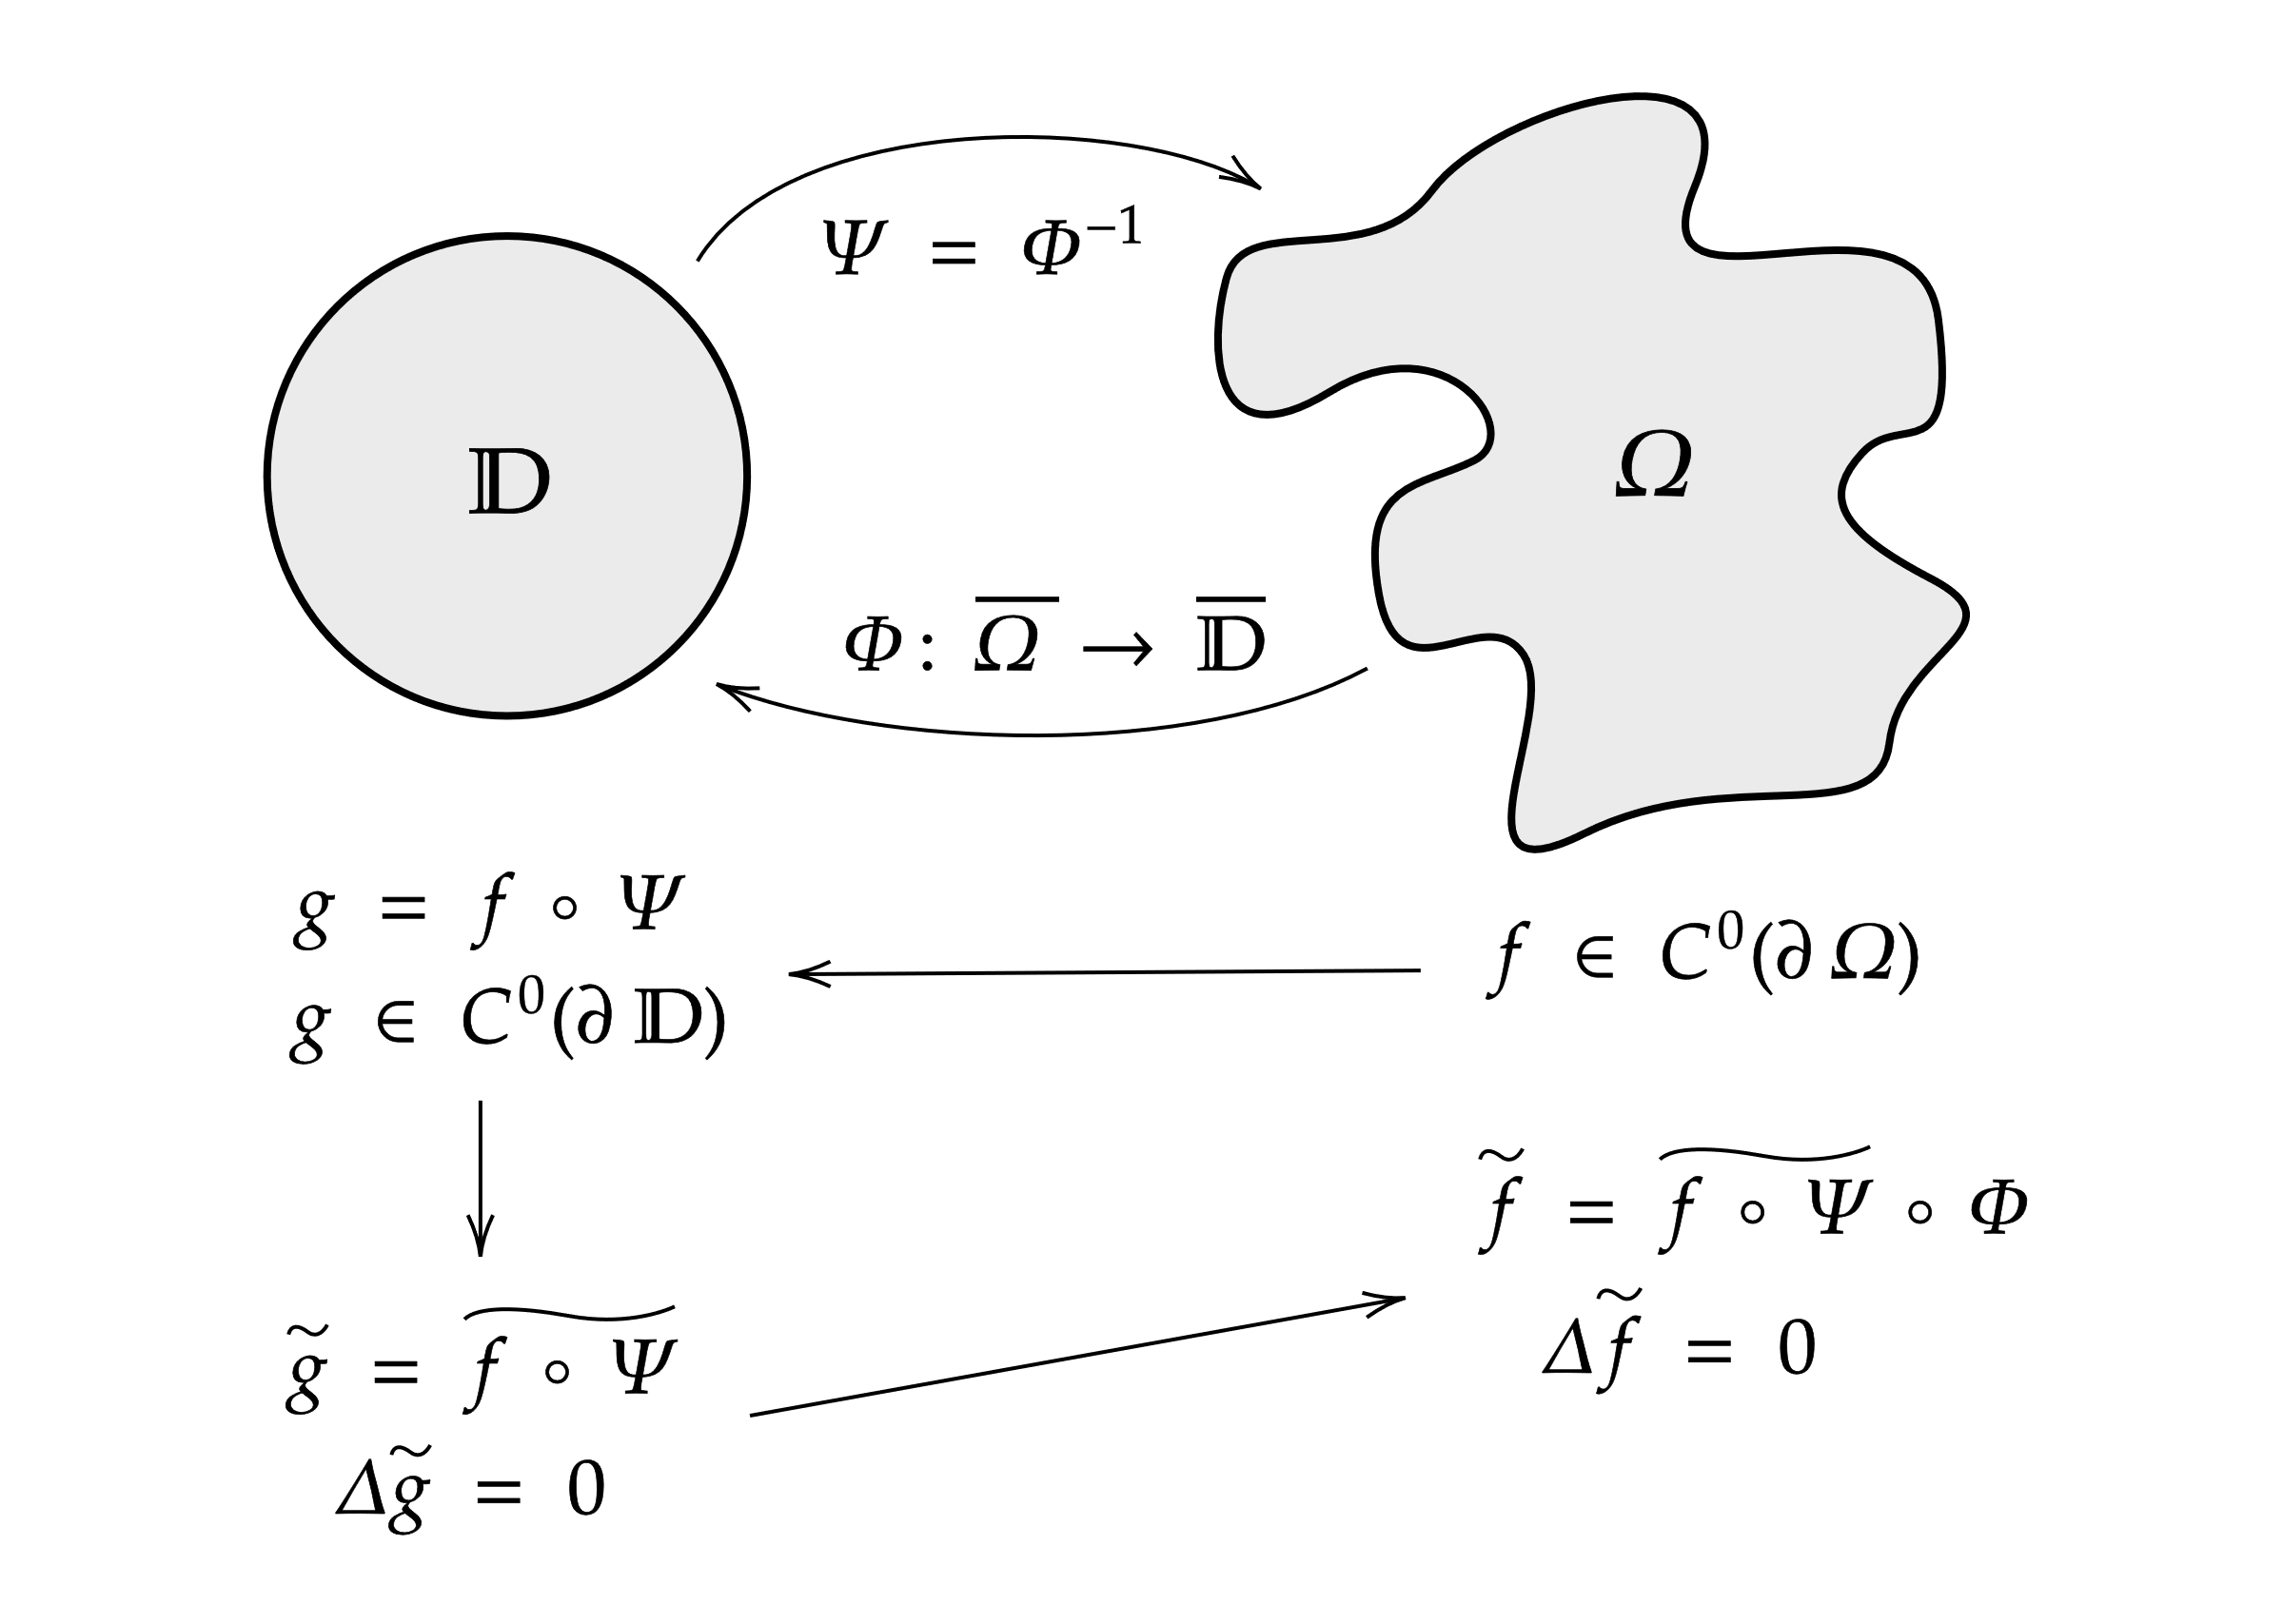
\includegraphics[width = \textwidth]{dirichlet_splosno.png}
            \caption{Izpeljava formule za rešitev Dirichletovega problema na omejenih enostavno povezanih območjih.}
        \end{center}    
    \end{figure}
    Sedaj si zgoraj zapisan predpis oglejmo na nekoliko bolj konkretnem primeru. 
    
    \begin{trditev}
        \label{alldisk}
        Naj bo $h$ zvezna funkcija, definirana na $\partial \mathbb{D}(a,R)$, kjer $a \in \mathbb{C}$ in $R>0$.  
        Za robni pogoj $h$ obstaja rešitev za Dirichletov problem na disku $\mathbb{D}(a,R)$ in je podana s predpisom
        $$
            H(a + r e^{i \theta}) = \begin{cases}
                    h(a + R e^{i \theta}),~~r = R,~\theta \in [0, 2\pi]\\
                    \widetilde{h}(a + r e^{i \theta}),~~ r \in [0,R),~ \theta \in [0, 2\pi]
            \end{cases},~\text{kjer}
        $$
        $$
        \widetilde{h}(a + r e^{i \theta}) = \int_{0}^{2 \pi}{h(a + R e^{i \varphi}) \left(\frac{R^2 - r^2}{R^2 + r^2 - 2Rr \cos(\theta - \varphi)}\right) \frac{d \varphi}{2 \pi}}.
        $$
     \end{trditev}
     \begin{dokaz}
        Pomagali si bomo zgoraj zapisanim postopkom za konstrukcijo rešitve za \mbox{Dirichletov} problem na omejenih enostavnih povezanih območjih. 
        Sedaj definirajmo $\Psi(z) = Rz + a,~z \in \overline{\mathbb{D}}$. Gre za biholomorfizem, katerega inverz je \mbox{$\Phi(\xi) = \frac{1}{R}(\xi - a)$}, $\xi \in \overline{\mathbb{D}}(a,R)$.
        Prek zapisa \eqref{eno_pov_obm} dobimo
        $$ 
        \widetilde{h}(\xi) = \frac{1}{2\pi i}\int_{\partial \mathbb{D}(a,R)}{h(\tau) \left(\frac{1 - |\frac{1}{R}(\xi - a)|^2}{|\frac{1}{R}(\tau - a) - \frac{1}{R}(\xi - a)|^2}\right)\frac{\frac{1}{R}}{\frac{1}{R}(\tau - a)}~d \tau}~,~~\xi \in \mathbb{D}(a,R). 
        $$
        Sedaj v integral uvedemo novo spremenljivko $\tau = a + Re^{i \varphi},~\varphi \in [0,2\pi]$, ter označimo $\xi = a + z,~z \in \mathbb{D}(0, R)$. Dobimo
        \begin{align*}
            \widetilde{h}(a + z) &= \frac{1}{2\pi i}\int_{0}^{2 \pi}{h(a + R e^{i \varphi}) \left(\frac{1 - \frac{1}{R}|z|^2}{|e^{i \varphi} - \frac{1}{R} z|^2}\right)~\frac{(i R e^{i \varphi}) d \varphi}{R e^{i \varphi}}}\\
            & = \frac{1}{2 \pi}\int_{0}^{2 \pi}{h(a + R e^{i \varphi}) \left(\frac{1 - \frac{1}{R}|z|^2}{|e^{i \varphi} - \frac{1}{R} z|^2}\right)~d\varphi}\\
            & = \frac{1}{2 \pi}\int_{0}^{2 \pi}{h(a + R e^{i \varphi}) \left(\frac{R^2 - |z|^2}{|R e^{i \varphi} - z|^2}\right)~d\varphi}~,~~z \in \mathbb{D}(0,R).
        \end{align*}
        Parametrizirajmo še $z \in \mathbb{D}(0,R)$, kot $z = r e^{i \theta},~r \in [0,R),~\theta \in [0,2 \pi]$. Sledi
        \begin{align*}
            \widetilde{h}(a + r e^{i \theta}) &= \frac{1}{2 \pi}\int_{0}^{2 \pi}{h(a + R e^{i \varphi}) \left(\frac{|R|^2 - |r e^{i \theta}|^2}{|R e^{i \varphi} - r e^{i \theta}|^2}\right)~d\varphi} \\
            & = \frac{1}{2 \pi}\int_{0}^{2 \pi}{h(a + R e^{i \varphi}) \left(\frac{R^2 - r^2}{R^2 - 2Rr \cos(\theta - \varphi) + r^2}\right)d\varphi},~r e^{i \theta} \in \mathbb{D}(0,R).
        \end{align*}
        Prišli smo do želenega predpisa na notranjosti diska $\mathbb{D}(a,R)$. 
        Očitno je, da razširitev zares reši Dirichletov problem na $\mathbb{D}(a,R)$ za robni pogoj $h$.
     \end{dokaz}

\subsection{Karakterizacija harmoničnih funkcij}
    Spomnimo se glavne motivacije za poglavje.
    Z znanjem, pridobljenim znotraj razdelka, je sedaj dokaz karakterizacije harmoničnih funkcij na dlani.
    
    \begin{trditev}
        \label{ekvhlp}
        Naj bo $h$ zvezna funkcija, definirana na območju $U \subseteq \mathbb{C}$. Velja, da je $h$ harmonična funkcija natanko tedaj, ko ima na $U$ lastnost povprečne vrednosti.
    \end{trditev}
    \begin{dokaz}
        Trditev \ref{harmonicnapovp} nam dokaže eno implikacijo. Dokazati je potrebno torej le še, da je zvezna funkcija $h$ z lastnostjo povprečne vrednosti na $U$ harmonična. 
        Dokaz temelji na obstoju rešitve Dirichletovega problema za poljuben disk. 
        
        Ker je $U$ območje, za poljubno točko $z_0 \in U$ obstaja $r>0$, da je $\overline{\mathbb{D}}(z_0,r) \subseteq U$. Ker je $h$ zvezna na $U$, $h$ na $\partial \overline{\mathbb{D}}(z_0, r)$ določa začetne pogoje za Dirichletov problem za disk $\mathbb{D}(z_0,r)$.
        Trditev \ref{obstoj} in \ref{alldisk} potrdita, da rešitev obstaja. Rešitev označimo s $H$.
        Kot harmonična funkcija na $\mathbb{D}(z_0, r)$, ima po trditvi \ref{harmonicnapovp} $H$ na $\mathbb{D}(z_0, r)$ lastnost povprečne vrednosti. 
        Oglejmo si sedaj funkcijo $g(z) = h(z) - H(z)$ za $z \in \overline{\mathbb{D}}(z_0,r)$. 
        Kot razlika funkcij z lastnostjo povprečne vrednosti ima tudi $g$ na $\mathbb{D}(z_0, r)$ lastnost povprečne vrednosti in je kot razlika dveh zveznih funkcij zvezna na $\overline{\mathbb{D}}(z_0, r)$.
        Vemo celo, da na $\partial \overline{\mathbb{D}}(z_0, r)$ velja $g \equiv 0$, saj je zožitev $H$ na $\partial \overline{\mathbb{D}}(z_0,r)$ enaka $h$. 
        Po posledici \ref{posledica_pm_lpv} je potem $g \equiv 0$ na $\overline{\mathbb{D}}(z_0, r)$, oziroma $H(z) =  h(z)$, za vsak $z \in \overline{\mathbb{D}}(z_0, r)$. Sledi, da je $h$ harmonična na $\mathbb{D}(z_0, r)$, oziroma ima poljubna točka $z_0$ v $U$ okolico, na kateri je $h$ harmonična. 
        Posledično je funkcija $h$ harmonična na $U$.
    \end{dokaz}
    \begin{posledica}
        Naj bo $u$ realna zvezna funkcija z lastnostjo povprečne vrednosti, definirana na območju $D$. Potem je $u$ na $D$ gladka, oziroma $u \in C^{\infty}(D)$.
    \end{posledica}
    \begin{dokaz}
        Po trditvi \ref{ekvhlp} je $u$ harmonična, po trditvi \ref{gladkost_komp_h} pa zato tudi gladka.
    \end{dokaz}

    Karakterizacija harmoničnih funkcij, prek lastnosti povprečne vrednosti, je primerljiva s karakterizacijo holomorfnih funkcij, ki jo ponuja izrek Morera. 
    Ta nam pove, da je na območju zvezna funkcija holomorfna natanko tedaj, ko je krivuljni integral funkcije po robu vsakega trikotniku, ki je v celoti vsebovan v območju, enak nič.
    Opazimo torej, da se za zvezne funkcije pojem harmoničnosti oziroma holomorfnosti izraža preko zahteve za krivuljni integral po robu (majhnega) diska oziroma robu trikotnika.
    Prednost obeh karakterizacij bo jasna znotraj naslednjega poglavja. Karakterizacija harmoničnih funkcij bo ključna pri dokazu Schwarzovega principa zrcaljenja za harmonične funkcije, 
    karakterizacija holomorfnih funkcij pa bo ključna za dokaz Schwarzovega principa zrcaljenja za holomorfne funkcije. 


\section{Schwarzov princip zrcaljenja}

Nekoliko se še navežimo na prejšno poglavje. 
Srečali smo se s problemom obstoja in konstrukcije razširitve, podane funkcije, ki bo obenem zadoščala zahtevam problema.  
Pri Dirichletovem problemu, smo zahtevali harmoničnost razširitve na notranjost in zveznost razširitve na zaprtju območja. 
Pokazali smo, da lahko na enotskem disku zahtevam problema, z robnim pogojem $h$, zadostimo s pomočjo Poissonovega integrala podane funkcije. Definirali smo razširitev
$$
    H(z) = 
    \begin{cases}
        h(z)~,~~&z \in \partial \mathbb{D} \\
        \widetilde{h}(z)~,~~&z \in \mathbb{D}
    \end{cases}.
$$

Sedaj si zastavimo nekoliko drugačen problem s podobnim ciljem. Ponovno poskusimo poiskati oziroma skonstruirati razširitev podane funkcije. 
Tokrat naj bo začetni podatek problema harmonična oziroma holomorfna funkcija, definirana na manjšem območju. Želeli bi poiskati harmonično oziroma holomorfno razširitev funkcije, ki bo definirana na novem območju podobne oblike.
Na hitro opisan problem bomo skozi poglavje rešili s pomočjo Schwarzovega principa zrcaljenja za harmonične oziroma holomorfne funkcije. 
Kaj točno smatramo za območje podobne oblike bo jasno v nadaljevanju, vendar kot to že nakazuje beseda zrcaljanje v imenu principa, bomo razširitev želeli konstruirati na zrcalni sliki prvotnega območja. 

\subsection{Definicije osnovnih pojmov}

    Spoznajmo najprej nekaj osnovnih pojmov, ki nam bodo omogočili natančno formulacijo in dokaz glavnega izreka poglavja.
    \begin{definicija}
        Naj bo $U \subseteq \mathbb{C}$ območje. Potem je $U^* = \{\overline{z}~|~z \in U\}$ \emph{zrcalna slika območja U glede na realno os}.
        Če za območje $U$ velja $U^* = U$ pravimo, da je območje $U$ \emph{simetrično glede na realno os}.
    \end{definicija}

    \begin{definicija}
        Naj bo $u$ funkcija, definirana na območju $U \subseteq \mathbb{C}$. Potem z \emph{$u^*$} označimo funkcijo, definirano na $U^*$, s predpisom $u^*(w) = \overline{u(\overline{w})},~w \in U^*$
    \end{definicija}

    Opazimo, da predpis iz zgornje definicije, za funkcijo $u$ definirano na območju $U$, ponuja zvezo $u^*(\overline{z}) = \overline{u(\overline{\overline{z}})} = \overline{u(z)},~z \in U$.
    Zapisana zveza nakazuje, da se bodo v veliki meri lastnosti funkcije $u$ prenesle na funkcijo $u^*$.

    \begin{opomba}
        Na tem mestu le spomnimo, da je za realne funkcije $u$, definirane na $U$, konjugiranje funkcijskih vrednosti pri predpisu funkcije $u^*$ odveč. Torej je funkcija $u^*$ določena kar prek zveze $u^*(w) = u(\overline{w}),~w \in U^*$.
    \end{opomba}

\subsection{Schwarzov princip zrcaljenja za harmonične funkcije}

    Pripravljeni smo na formulacijo in dokaz glavnega izreka. 

    \begin{lema}
        \label{lemaharm}
        Naj bo $u$ realna funkcija, definirana na območju $U \subseteq \mathbb{C}$. Če je $u$ harmonična na $U$, potem je $u^*$ harmonična na $U^*$. 
    \end{lema}
    \begin{proof}
        Trditev dokažimo na dva načina. Dokaz prvega načina temelji na uporabi karakterizacije harmoničnih funkcij z lastnostjo povprečne vrednosti. 
        
        Naj bo \mbox{$w_0 \in U^*$}. Ker je $U^*$ območje, obstaja $\rho>0$, da za vsak $0 < r < \rho$ velja $\overline{\mathbb{D}}(w_0, r) \subseteq U^*$. Po definiciji $U^*$ sledi, da za vsak \mbox{$0 < r < \rho$} velja $\overline{\mathbb{D}}(\overline{w_0}, r) \subseteq U$. 
        Ker je funkcija $u$ na $U$ harmonična, ima po trditvi \ref{ekvhlp} na $U$ lastnost povprečne vrednosti. Sledi
        \begin{align*}
            u^*(w_0) & = u(\overline{w_0}) = \frac{1}{2 \pi} \int_{0}^{2 \pi}{u\left(\overline{w_0} + r e^{i \theta}\right) d\theta} = \frac{1}{2 \pi} \int_{0}^{2 \pi}{u\left(\overline{w_0 + r e^{-i \theta}}\right) d\theta}\\
            &= \frac{1}{2 \pi} \int_{0}^{2 \pi}{u^*\left(w_0 + r e^{-i \theta}\right) d\theta} = \frac{1}{2 \pi} \int_{0}^{2 \pi}{u^*\left(w_0 + r e^{i \theta}\right) d\theta},~r \in (0, \rho).
        \end{align*} 
        Pokazali smo, da ima funkcija $u^*$ na $U^*$ lastnost povprečne vrednosti. 
        Ker je funkcija $u$ zvezna na $U$, je očitno funkcija $u^*$ zvezna na $U^*$. 
        Po trditvi \ref{ekvhlp} sledi, da je funkcija $u^*$ na $U^*$ harmonična. 
        
        Dokažimo trditev še po definiciji, tj. dokažimo, da $u^*$ na $U^*$ zadošča Laplaceovi parcialni diferencialni enačbi.
        Pomagali si bomo z standardno identifikacijo kompleksne spremenljivke $z = x + iy$ s parom realnega in imaginarnega dela $(x,y)$.
        Identifikacija nam narekuje zvezo $u^*(x,-y) = u(x, y),~ x + iy \in U$.
        Sedaj parcialno odvajajmo in dobimo
        \begin{align*}
            \frac{\partial u}{\partial x} &= \frac{\partial u^* }{\partial x}~,~~~~~\frac{\partial u}{\partial y} = - \frac{\partial u^* }{\partial y}, \\
            \frac{\partial^2 u}{\partial x^2} & = \frac{\partial^2 u^* }{\partial x^2}~,~~~~~\frac{\partial^2 u}{\partial y^2} = \frac{\partial^2 u^* }{\partial y^2}.
        \end{align*}
        Ker je funkcija $u$ na $U$ harmonična, velja
        $$
            \Delta u^* = \frac{\partial^2 u^*}{\partial x^2} + \frac{\partial^2 u^*}{\partial y^2} = \frac{\partial^2 u}{\partial x^2} + \frac{\partial^2 u}{\partial y^2} = 0.
        $$
        Sledi, da je $u^*$ harmonična na $U^*$.
    \end{proof}
    
    \begin{izrek}[Schwarzov princip zrcaljenja za harmonične funkcije]
        \label{schwarz_harm}
        Naj bo $D \subseteq \mathbb{C}$ območje, simetrično glede na realno os. 
        Označimo $D^{+} = \{z \in D~|~\text{Im}[z] > 0\},~D^{-} = \{z \in D~|~\text{Im}[z] < 0\}$ in $D^{0} = \{z \in D~|~\text{Im}[z] = 0\}$.
        Naj bo $u$ realna zvezna funkcija, definirana na $D^{+} \cup D^0$. Naj bo $u$ na $D^{+}$ harmonična in naj za vsak $z \in D^0$ velja $u(z) = 0$.
        Potem obstaja harmonična razširitev funkcije $u$ na $D$, ki je eksplicitno podana prek zveze $u(\bar{z}) = - u(z),~z \in D$.
    \end{izrek}

    V trditvi zapisano situacijo komentirajmo še s pomočjo spodnje slike. 
    \begin{figure}[H]
        \begin{center}
            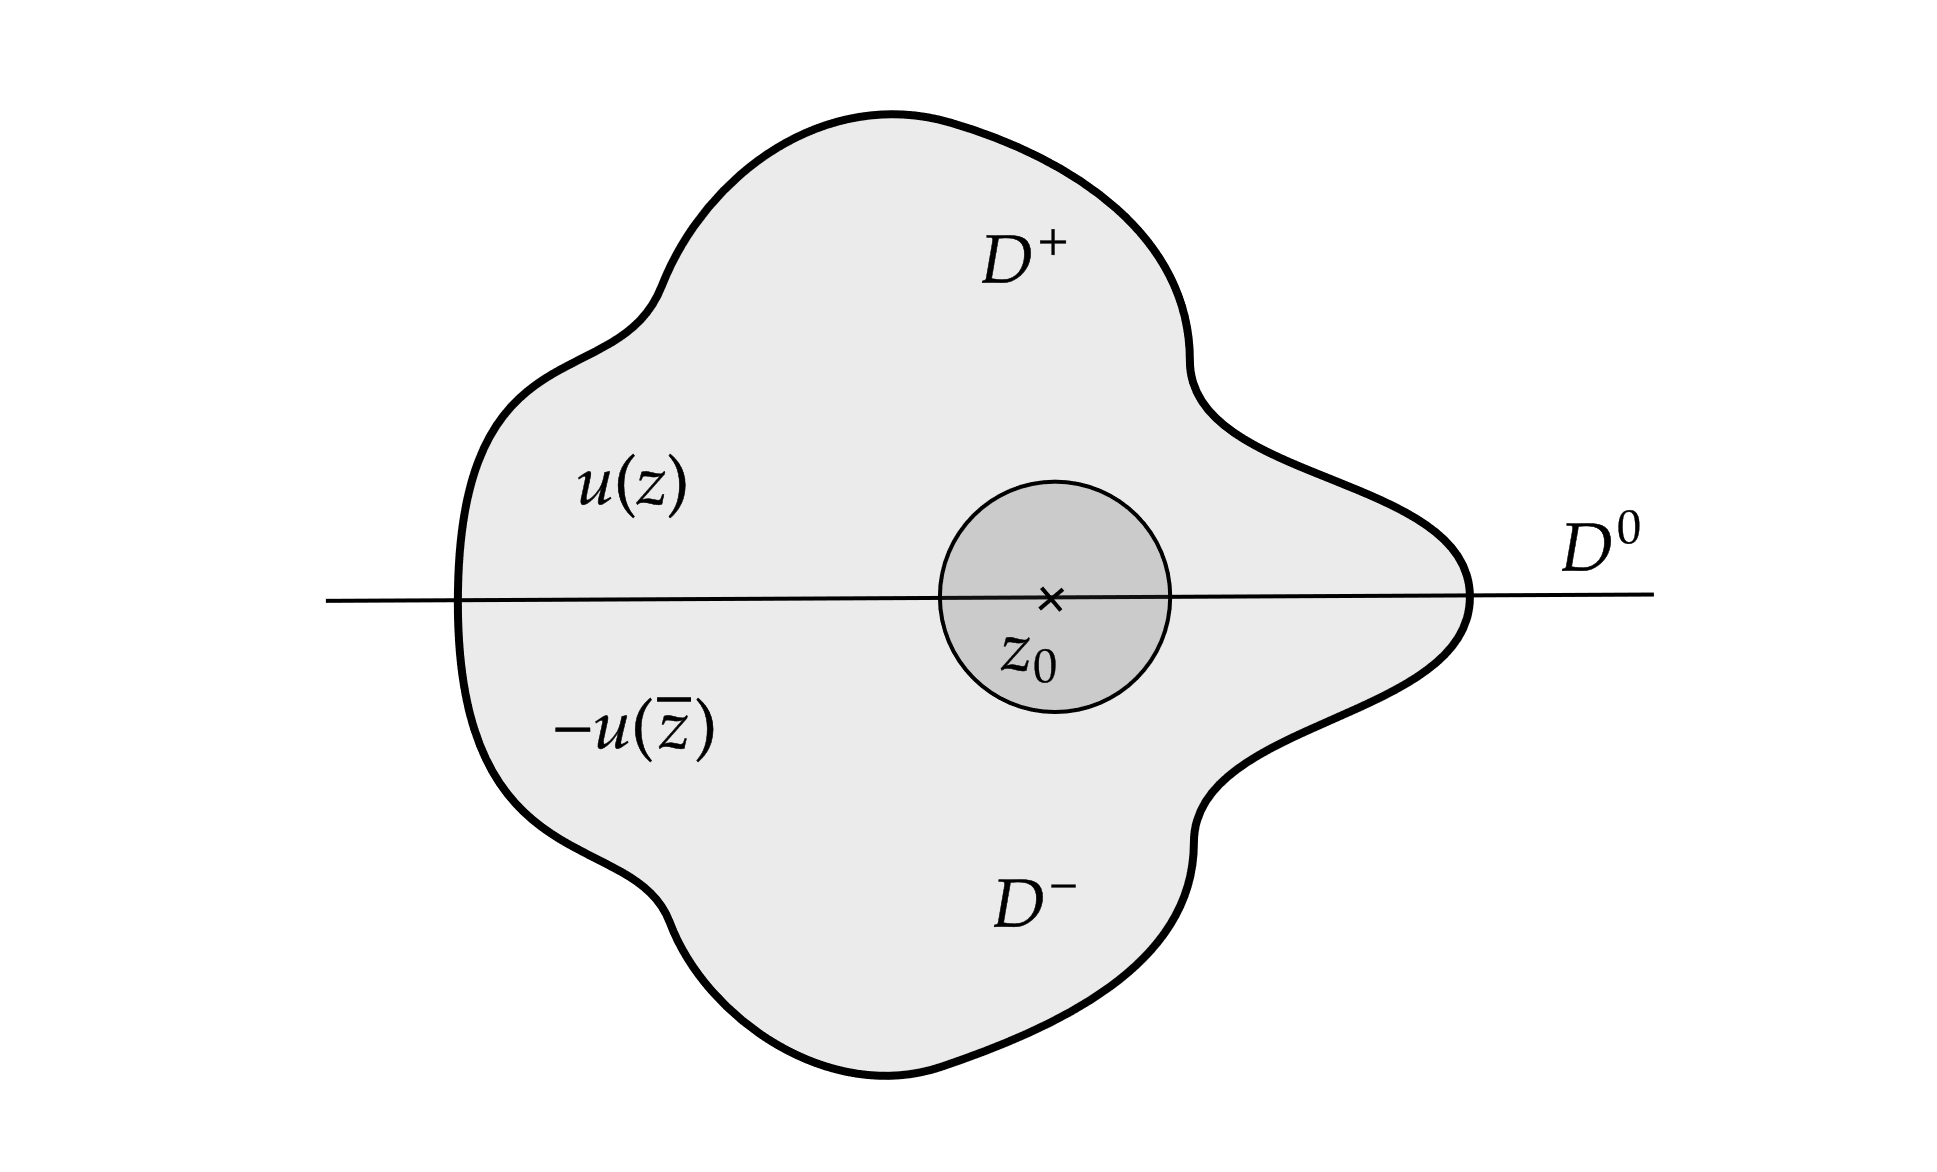
\includegraphics[width = \textwidth]{schwarz_harm.png}
            \caption{Schwarzov princip zrcaljenja za harmonične funkcije.}
        \end{center}    
    \end{figure}

    Slika prikazuje glede na realno os simetrično območje $D \subseteq \mathbb{C}$. $D^{+}$ označuje območje, na katerem je poznana funkcija $u$ harmonična, $D^{-}$ pa zrcalno sliko območja $D^+$ glede na realno os. 
    Predpis razširitve je na $D^-$ podan s predpisom \mbox{$u(\overline{z}) = - u(z)$}.
    Vodoravna črta prikazuje odsek realne osi. Odsek, ki leži znotraj območja $D$ smo označili z $D^0$. Funkcija $u$ je na tem delu območja po predpostavki izreka ničelna.
    Točka $z_0$ in majhen disk okoli nje nakazujeta, da se bomo dokaza trditve lotili prek karakterizacije harmoničnih funkcij z lastnostjo povprečne vrednosti.

    \begin{dokaz}
        Opazimo, da je $D$ disjunktna unija $D^+$, $D^-$ in $D^0$.
        Na območju $D$ definirajmo funkcijo $U$, katere predpis narekuje eksplicitna zveza iz trditve
        $$
        U(z) = 
        \begin{cases}
            u(z)~,~~&z \in D^{+}\\
            -u(\overline{z})~,~~&z \in D^{-}\\
            0~,~~ &z \in D^0
        \end{cases}
        .
        $$
        Funkcija $U$ je po predpostavkah izreka zvezna na $D^+ \cup D^0$, iz definicije, prek predpisa $u(\overline{z}) = - u(z)$, pa je jasno, da je zvezna kar na $D$. 
        Posvetimo se dokazu harmoničnosti.
        Ker je $U$, oziroma $u$, na $D^+$ harmonična, ima po trditvi \ref{ekvhlp}, na $D^+$ lastnost povprečne vrednosti. 

        Opazimo, da funkcijski predpis funkcije $U$ na območju $D^-$ sovpada s predpisom funkcije $- u^*(z)$. 
        Ker je $U$, oziroma $u$, na $D^+$ harmonična, je po lemi \ref{lemaharm} $-u^*(z)$, oziroma $U$ harmonična na $(D^+)^* = D^-$.
        Po trditvi \ref{ekvhlp} ima $U$ na $D^-$ lastnost povprečne vrednosti. 
        
        Sedaj nam preostane le še $D^0$.
        Vzemimo poljubno točko $z_0 \in D^0 \subseteq \mathbb{R}$. Ker je $D$ območje, obstaja $\rho > 0$, da je $\overline{\mathbb{D}}(z_0, \rho) \subseteq D$. Za vsak $0 < r < \rho$ velja
        \begin{align*}
            \frac{1}{2 \pi} \int_{0}^{2 \pi}{U(z_0 + re^{i \theta}) d\theta} &= \frac{1}{2 \pi} \left(\int_{0}^{\pi}U(z_0 + re^{i \theta})~d\theta + \int_{\pi}^{2\pi} U(z_0 + re^{i \theta})~d\theta\right) \\
            & = \frac{1}{2 \pi} \left(\int_{0}^{\pi}U(z_0 + re^{i \theta})~d\theta + \int_{0}^{\pi}U(\overline{z_0 + re^{i \theta}})~d\theta\right) \\
            &= \frac{1}{2 \pi} \left(\int_{0}^{\pi}u(z_0 + re^{i \theta})~d\theta - \int_{0}^{\pi}u(z_0 + re^{i \theta})~d\theta\right) = 0.
        \end{align*}        
        Ker je funkcija $U$ na $D^0$ ničelna, smo pokazali, da ima $U$ tudi na $D^0$ lastnost povprečne vrednosti. 
        Dokazali smo, da ima zvezna funkcija $U$ na $D = D^+ \cup D^- \cup D^0$ lastnost povprečne vrednosti, zato je po trditvi \ref{ekvhlp} na $D$ harmonična.
    \end{dokaz}

\subsection{Schwarzov princip zrcaljenja za holomorfne funkcije}

    Schwarzov princip zrcaljenja lahko formuliramo in dokažemo tudi za holomorfne funkcije. 
    Postopajmo podobno kot v prejšnem razdelku.

    \begin{lema}
        \label{lemahol}
        Naj bo $f$ holomorfna funkcija, definirana na območju $U \subseteq \mathbb{C}$.
        Potem je funkcija $f^*$ holomorfna na $U^*$.
    \end{lema}
    \begin{dokaz}
        Trditev ponovno dokažimo na dva načina. Dokaza se najprej lotimo s pomočjo Cauchy-Riemannovega sistema, nato pa holomorfnost funkcije $f^*$ dokažimo še po definiciji.

        Označimo $f(z) = u(z) + iv(z),~ z \in U$ in $f^*(w) = p(w) + iq(w),~w \in U^*$, kjer so $u,v, p$ in $q$ realne funkcije. 
        Iz definicije funkcije $f^*$ sledi $f^*(w) = \overline{u(\overline{w}) + iv(\overline{w})} = u(\overline{w}) - iv(\overline{w}),~ w \in U^*$. 
        Sedaj enačimo realni in imaginarni del zapisanih funkcij. Dobimo
        \begin{align*}
            p(w) &= u(\overline{w}),~w \in U^*~,~~\text{oziroma}~~~~p(\overline{z}) = u(z),~z \in U~,~~\text{ter} \\
            q(w) &= -v(\overline{w}),~w \in U^*~,~~\text{oziroma}~~~~q(\overline{z}) = -v(z),~z \in U.
        \end{align*}
        Enakosti lahko sedaj ob upoštevanju identifikacije $z \leftrightarrow (x,y)$ oziroma $\overline{z} \leftrightarrow (x, -y)$ parcialno odvajamo po realnih spremenljivkah $x$ in $y$. Dobimo
        \begin{align*}
            \frac{\partial u}{\partial x} &= \frac{\partial p}{\partial x}~~~~\text{in}~~~~ -\frac{\partial v}{\partial x} = \frac{\partial q}{\partial x}~,~~\text{ter}\\
            \frac{\partial u}{\partial y} &=  - \frac{\partial p}{\partial y}~~~~\text{in}~~~~ -\frac{\partial v}{\partial y} = - \frac{\partial q}{\partial y} \iff \frac{\partial v}{\partial y} = \frac{\partial q}{\partial y}~.      
        \end{align*}
        Ker je funkcija $f$ holomorfna, zadošča Cauchy-Riemannovemu sistemu enačb.  
        Sledi
        \begin{align*}
            \frac{\partial p}{\partial x} = \frac{\partial u}{\partial x} &= \frac{\partial v}{\partial y} = \frac{\partial q}{\partial y}~~~~\text{in}~~~~ \frac{\partial p}{\partial y} = -\frac{\partial u}{\partial y} = \frac{\partial v}{\partial x} = -\frac{\partial q}{\partial x}.
        \end{align*}
        Opazimo, da funkcija $f^* = p + iq$ zadošča Cauchy-Riemannovemu sistemu enačb, zato je holomorfna.

        Sedaj dokažimo holomorfnost funkcije $f^*$ še po definiciji. Želimo dokazati, da je $f^*$ v vsaki točki $w \in U^*$ kompleksno odvedljiva. Predpostavka trditve nam pove, da je $f$ kompleksno odvedljiva v vsaki točki $\overline{w} \in U$.
        Naj bo $w \in U^*$. Potem velja
        \begin{align*}
            \lim_{h \to 0}{~\frac{f^*(w + h) - f^*(w)}{h}} &= \lim_{h \to 0}{~\frac{\overline{f\left(\overline{w + h}\right)} - \overline{f(\overline{w})}}{h}} = \lim_{h \to 0}{~\overline{\frac{f\left(\overline{w + h}\right) - f(\overline{w})}{\overline{h}}}} \\
            \lim_{h \to 0}{~\overline{\frac{f\left(\overline{w} + \overline{h}\right) - f(\overline{w})}{\overline{h}}}} & = \overline{\lim_{\overline{h} \to 0}{~\frac{f\left(\overline{w} + \overline{h}\right) - f(\overline{w})}{\overline{h}}}} = \overline{f'(\overline{w})}.
        \end{align*}
        Limita diferenčnega kvocienta obstaja v poljubni točki $w \in U^*$, zato je $f^*$ na $U^*$ kompleksno odvedljiva oziroma holomorfna.
    \end{dokaz}

    \begin{trditev}[Schwarzov princip zrcaljenja za holomorfne funkcije]
        Naj bo $D \subseteq \mathbb{C}$ območje, simetrično glede na realno os. 
        Označimo $D^{+} = \{z \in D~|~\text{Im}[z] > 0\},~D^{-} = \{z \in D~|~\text{Im}[z] < 0\}$ in $D^{0} = \{z \in D~|~\text{Im}[z] = 0\}$.
        Naj bo $f$ zvezna funkcija, definirana na $D^{+} \cup D^0$. Naj bo $f$ na $D^{+}$ holomorfna in naj $f$ na $D^0$ zavzame realne vrednosti.
        Potem je funkcija $F$, definirana s predpisom
        $$
        F(z) = 
        \begin{cases}
            f(z)~,~~&z \in D^{+} \cup D^0\\
            f^*(z)~,~~&z \in D^{-} \cup D^0
        \end{cases}~,
        $$
        na območju $D$ holomorfna.
    \end{trditev}
    \begin{dokaz}
        Opazimo, da imata veji predpisa funkcije $F$ neprazen presek, zato se je smiselno vprašati, ali je predpis sploh dobro definiran. Potrebno je preveriti, ali se funkcijske vrednosti na preseku vej, oziroma $D^0$, ujemajo.  
        Ker za $z_0 \in D^0$ velja $\overline{z_0} = z_0$, funkcija $f$ pa po predpostavki trditve na $D^0$ zavzame realne vrednosti, sledi $f(z_0) = f(\overline{z_0}) = \overline{f(\overline{z_0})} = f^*(z_0)$.
        
        Območje $D$ je disjunktna unija $D^+$, $D^-$ in $D^0$. Vemo da je funkcija $F$, oziroma $f$, holomorfna na $D^+$, zato je po lemi \ref{lemahol} funkcija $f^*$, oziroma $F$, holomorfna na $(D^+)^* = D^-$. 
        Dovolj je torej dokazati, da je $F$ holomorfna v okolici vsake točke iz $D^0$. 
        Naj bo $z_0 \in D^0$ in $\delta > 0$ tak, da velja $\overline{\mathbb{D}}(z_0,\delta) \subseteq D$. Sedaj uporabimo karakterizacijo holomorfnih funkcij prek izreka Morera. 
        Funkcija $F$ je očitno zvezna kar na $D$, zato je dovolj pokazati, da za vsak zaprt trikotnik $T$, za katerega velja $T \subseteq \mathbb{D}(z_0, \delta)$ sledi
        $$ 
            \int_{\partial T}{F(\xi)~d\xi} = 0.
        $$
        Naj bo $T$ poljuben zaprt trikotnik, ki je v celoti vsebovan v $\mathbb{D}(z_0,\delta)$. Opazimo, da imamo dve možnosti.
        Bodisi je $T$ v celoti vsebovan v $\mathbb{D}(z_0,\delta) \cap D^+$ ali $\mathbb{D}(z_0,\delta) \cap D^-$, bodisi ima z $D^0$ neprazen presek. Sedaj možnosti ločimo.
        
        Če je $T$ v celoti vsebovan v $\mathbb{D}(z_0,\delta) \cap D^+$ ali $\mathbb{D}(z_0,\delta) \cap D^-$, nam holomorfnost funkcije $F$ na $D^+$ in $D^-$ omogoča uporabo Cauchyjevega izreka. 
        Ta nam pove, da je krivuljni integral po robu $T$ res enak nič. 
        Zapisana situacija je za zaprte trikotnike $T_1 \subseteq \mathbb{D}(z_0,\delta) \cap D^+$, ter zaprte trikotnike $T_2 \subseteq \mathbb{D}(z_0,\delta) \cap D^-$, grafično prikazana na spodnji sliki. 
        \begin{figure}[H]
            \begin{center}
                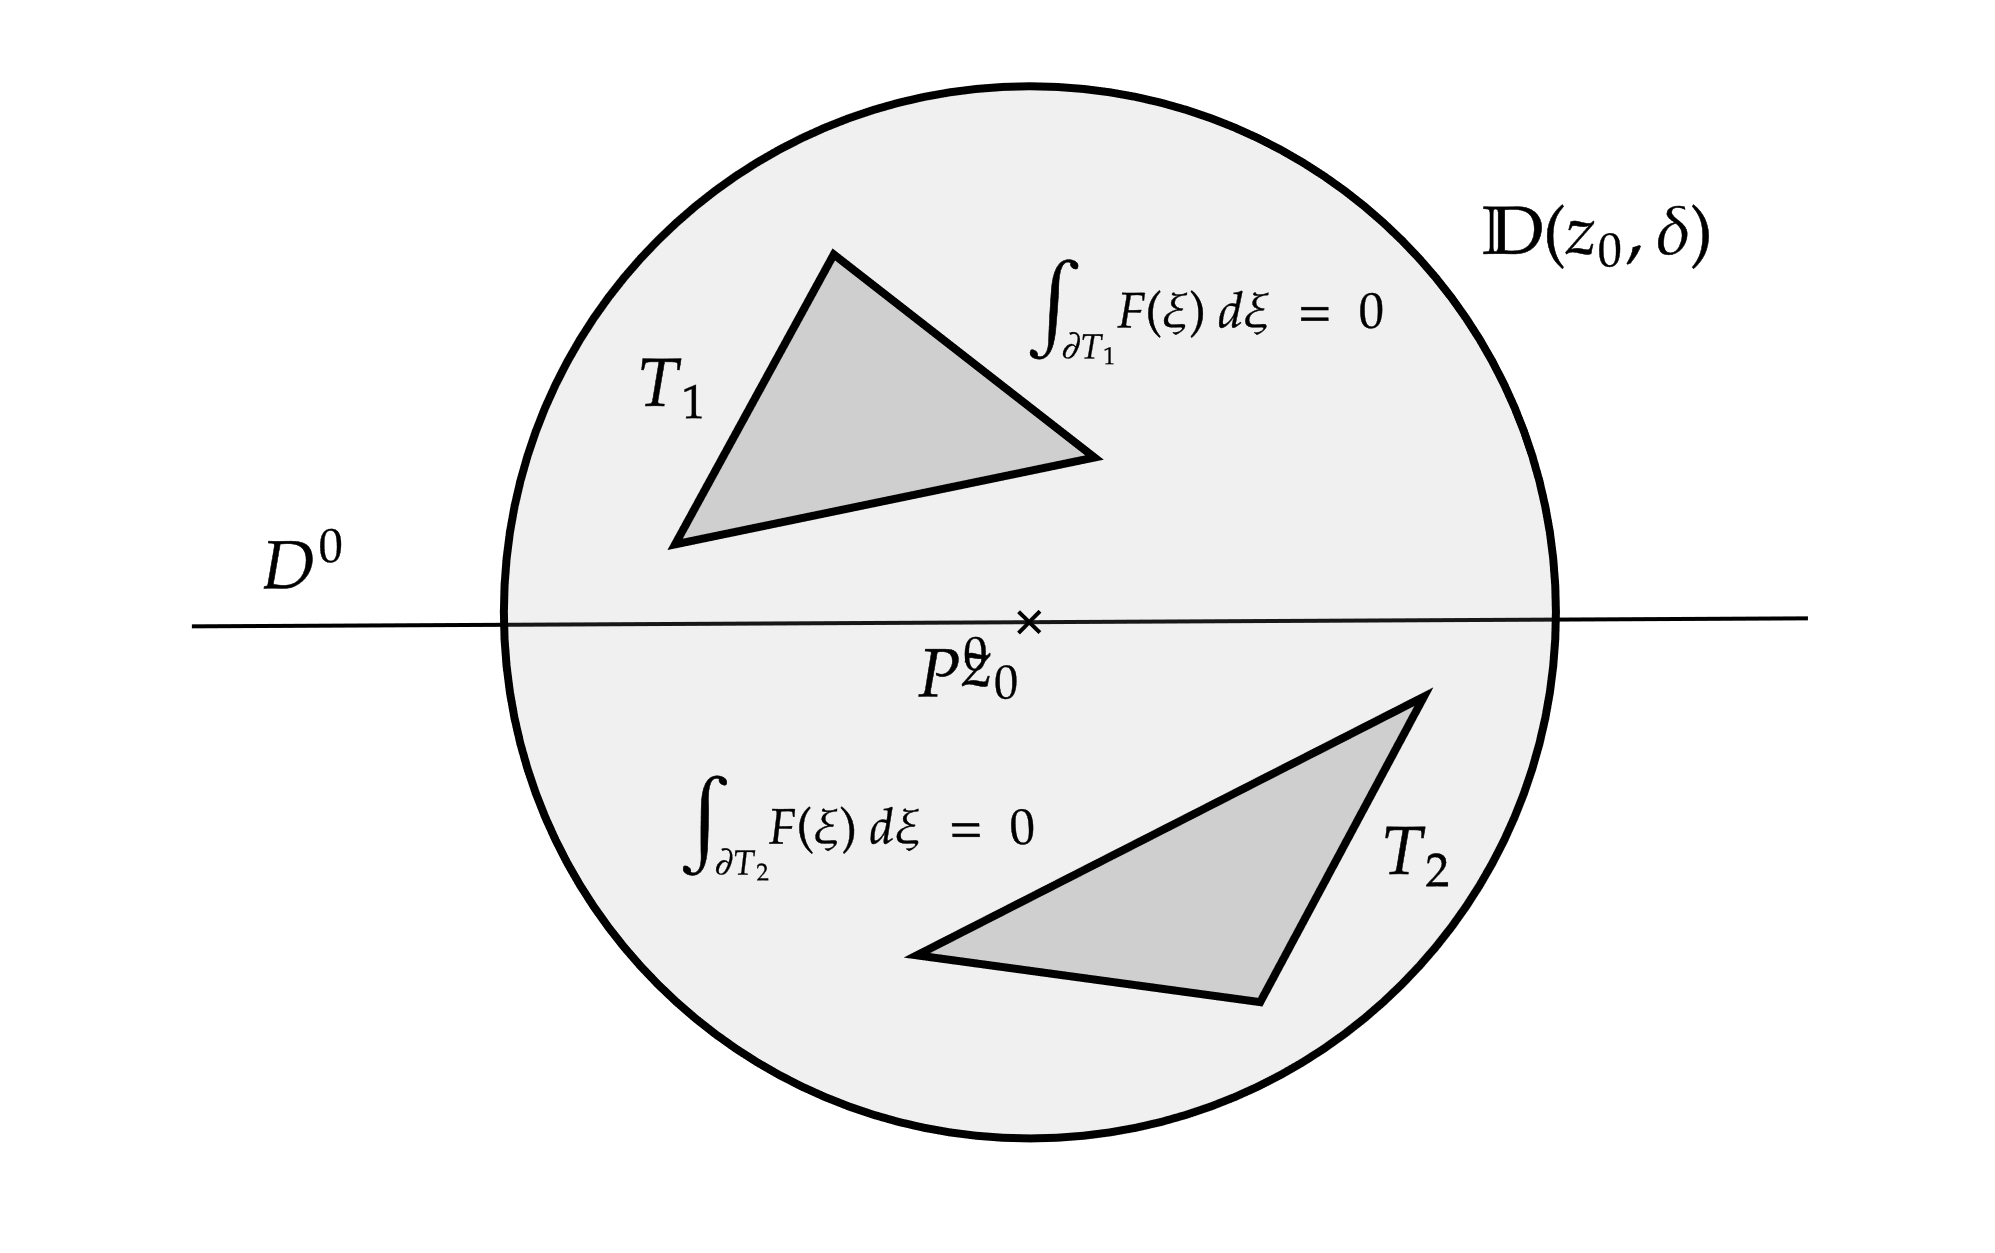
\includegraphics[width = 0.9 \textwidth]{schwarz_hol_1.png}
                \caption{Zaprta trikotnika $T_1$ in $T_2$, vsebovana v $\mathbb{D}(z_0,\delta) \cap D^+$ oziroma v $\mathbb{D}(z_0,\delta) \cap D^-$.}
            \end{center}    
        \end{figure}

        Posvetimo se drugi možnosti, torej možnosti, da presek zaprtega trikotnika $T$ in $D^0$ ni prazen. Brez škode za splošnost lahko predpostavimo, da eno oglišče leži nad realno osjo in preostali oglišči ležita pod realno osjo.
        Ideja je krivuljni integral po robu trikotnika prek $\delta_0 > 0$ dovolj blizu $D^0$ razbiti na krivuljna integrala, ki bosta v celoti znotraj območij $\mathbb{D}(z_0,\delta) \cap D^+$ oziroma $\mathbb{D}(z_0,\delta) \cap D^-$, 
        ter na krivuljni integral, katerega prispevek bo dovolj majhen.
        Sedaj definirajmo $P^+ = \{z \in T~|~\text{Im}[z] \geq \delta_0\}$, $P^- = \{z \in T~|~\text{Im}[z] \leq -\delta_0\}$ in $P^0 = \{z \in T~|~|\text{Im}[z]| \leq \delta_0\}$ ter si situacijo oglejmo grafično.

        \begin{figure}[H]
            \begin{center}
                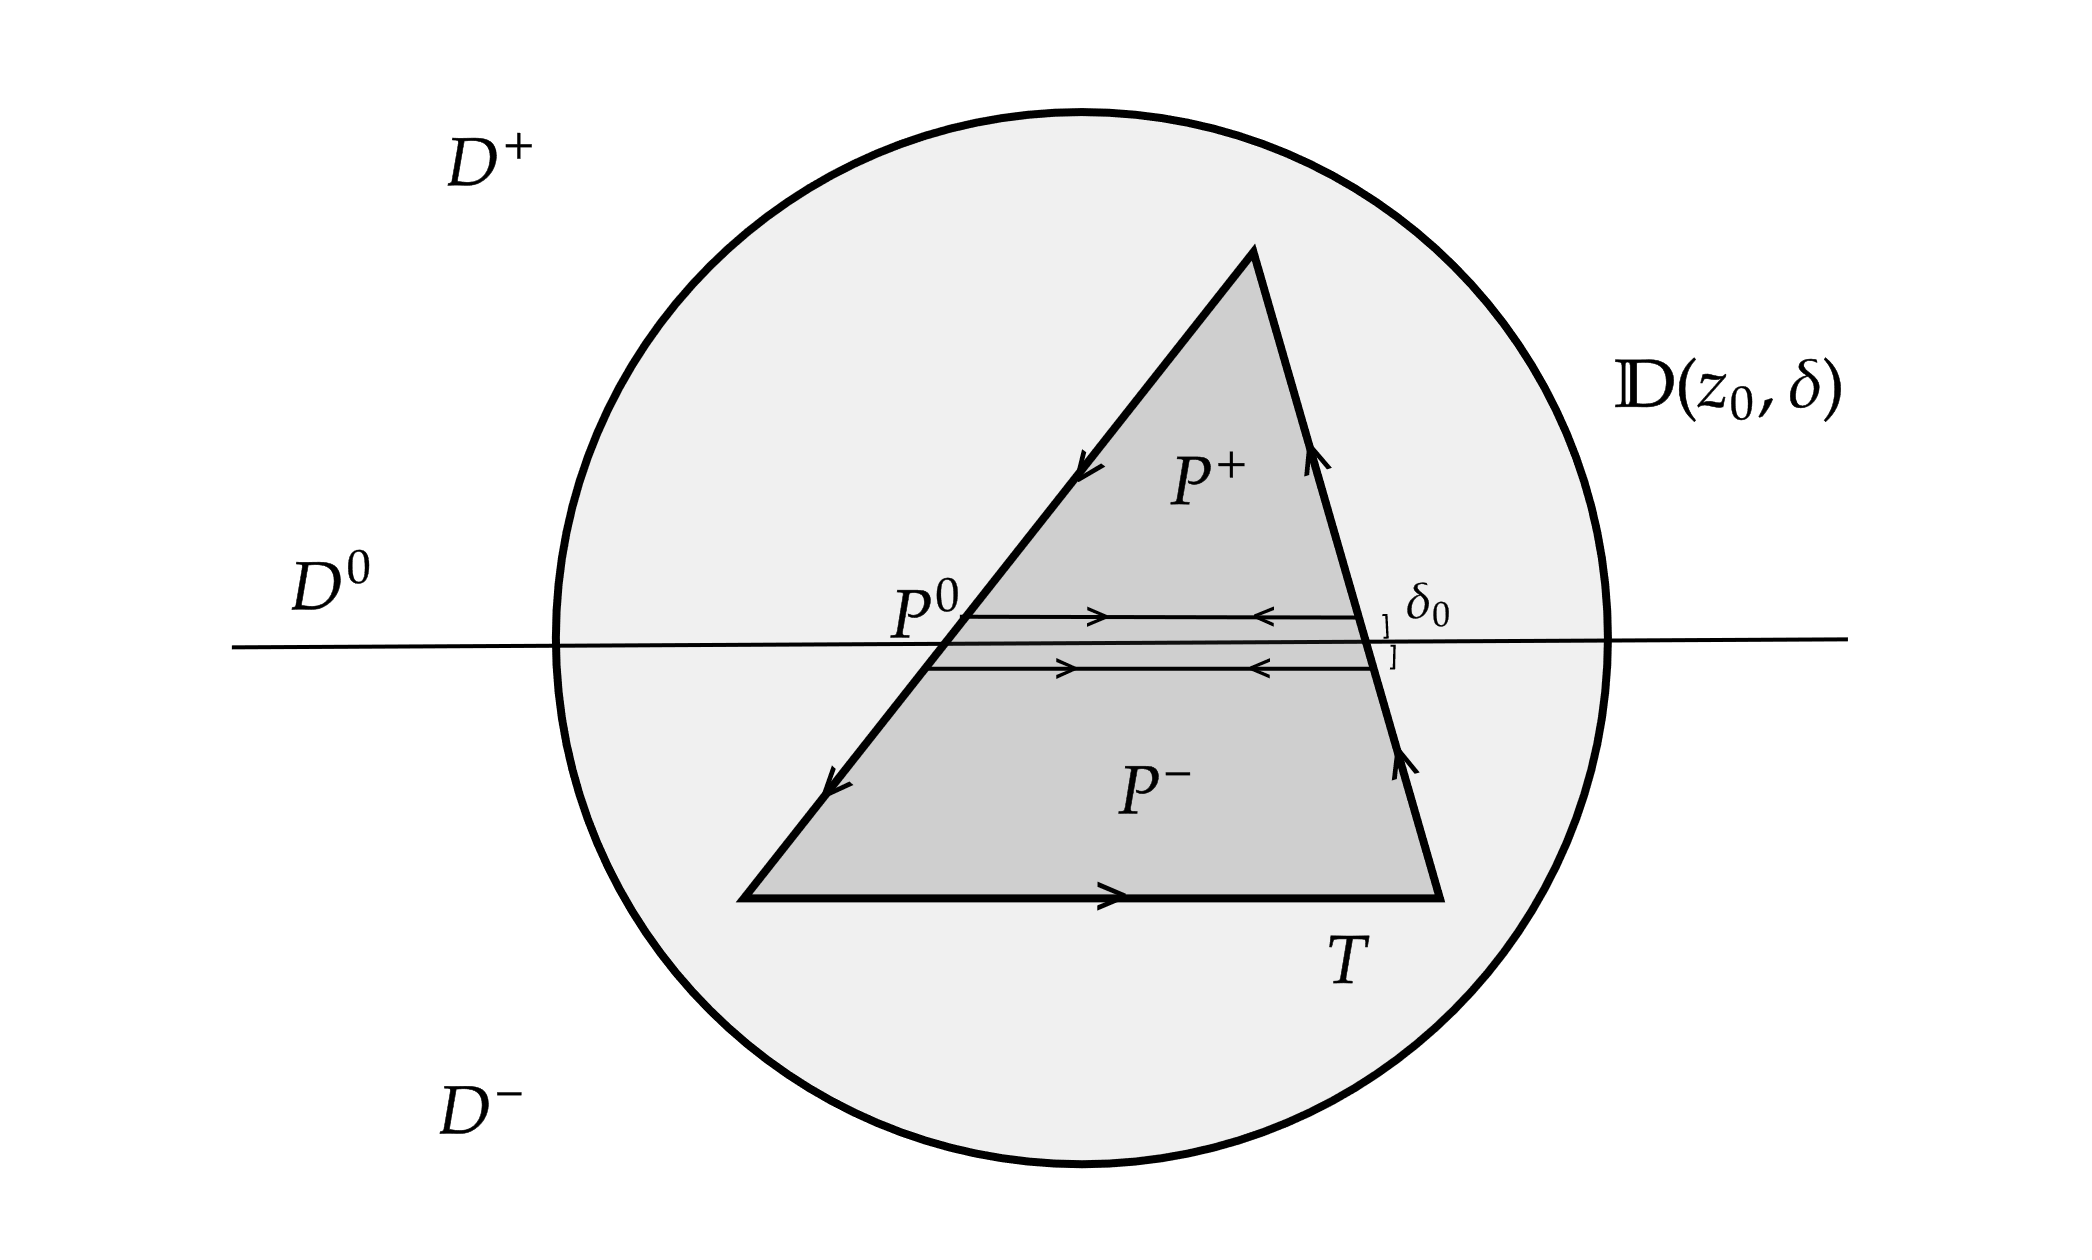
\includegraphics[width = 0.9 \textwidth]{schwarz_hol_2.png}
                \caption{Delitev zaprtega trikotnika $T$ na $P^+$, $P^-$ in $P^0$.}
            \end{center}    
        \end{figure}
        
        Naj bo $\epsilon > 0$. Želimo najti dovolj majhen $\delta > \delta_0 > 0$, za katerega bo delitev zaprtega trikotnika $T$ na $P^+$, $P^-$ in $P^0$ zadoščala
        $$ 
            \left|\int_{\partial P^0}{F(\xi)~d\xi}\right| < \epsilon~,~\text{ter zato po Cauchyjevem izreku za funkcijo $F$ na $P^+$ in $P^-$}
        $$
        \begin{align*}
            \left|\int_{\partial T}{F(\xi)~d\xi}\right| &= \left|\int_{\partial P^+}{F(\xi)~d\xi} + \int_{\partial P^-}{F(\xi)~d\xi} + \int_{\partial P^0}{F(\xi)~d\xi}\right|\\
            &\leq \left|\int_{\partial P^+}{F(\xi)~d\xi} \right|+ \left|\int_{\partial P^-}{F(\xi)~d\xi}\right| + \left|\int_{\partial P^0}{F(\xi)~d\xi}\right| \\ 
            & =\left|\int_{\partial P^0}{F(\xi)~d\xi} \right| < \epsilon.
        \end{align*}
        Sedaj razbijmo še krivuljni integral po $\partial P^0$. 
        Z $z_{ZL}$ oziroma $z_{ZD}$ označimo levo oziroma desno točko v preseku $\partial P^0$ in $\partial P^+$. 
        Podobno z $z_{SL}$ oziroma $z_{SD}$ označimo levo oziroma desno točko v preseku $\partial P^0$ in $\partial P^-$.
        S pomočjo $\delta_0 > 0$ označimo še $z_1 = z_{ZL} - 2 \delta_0$ in $z_2 = z_{ZD} - 2 \delta_0$.
        Označene točke nam ponujajo razbitje roba na neorientirane daljice. Označimo 
        \begin{align*}
            S_Z &= \{(1-t)z_{ZD} + t z_{ZL}~|~ t \in [0,1]\}, \\
            S_D &= \{(1-t)z_{ZL} + t z_{SL}~|~ t \in [0,1]\}, \\
            S_L &= \{(1-t)z_{SD} + t z_{ZD}~|~ t \in [0,1]\}~\text{in}\\ 
            S_S &= \{(1-t)z_{SL} + t z_{SD}~|~ t \in [0,1]\}.
        \end{align*}
        Nadaljno lahko daljico $S_S$ razdelimo na neorientirane daljice 
        \begin{align*}
            &S_1 = \{(1-t)z_{SL} + t z_{1}~|~ t \in [0,1]\}, \\
            &S_2 = \{(1-t)z_{2} + t z_{SD}~|~ t \in [0,1]\}~\text{in} \\
            &S_{S'} = \{(1-t)z_{1} + t z_{2}~|~ t \in [0,1]\}.
        \end{align*}
        Pred nadaljevanjem si zapisane oznake oglejmo na spodnji sliki. 
        \begin{figure}[H]
            \begin{center}
                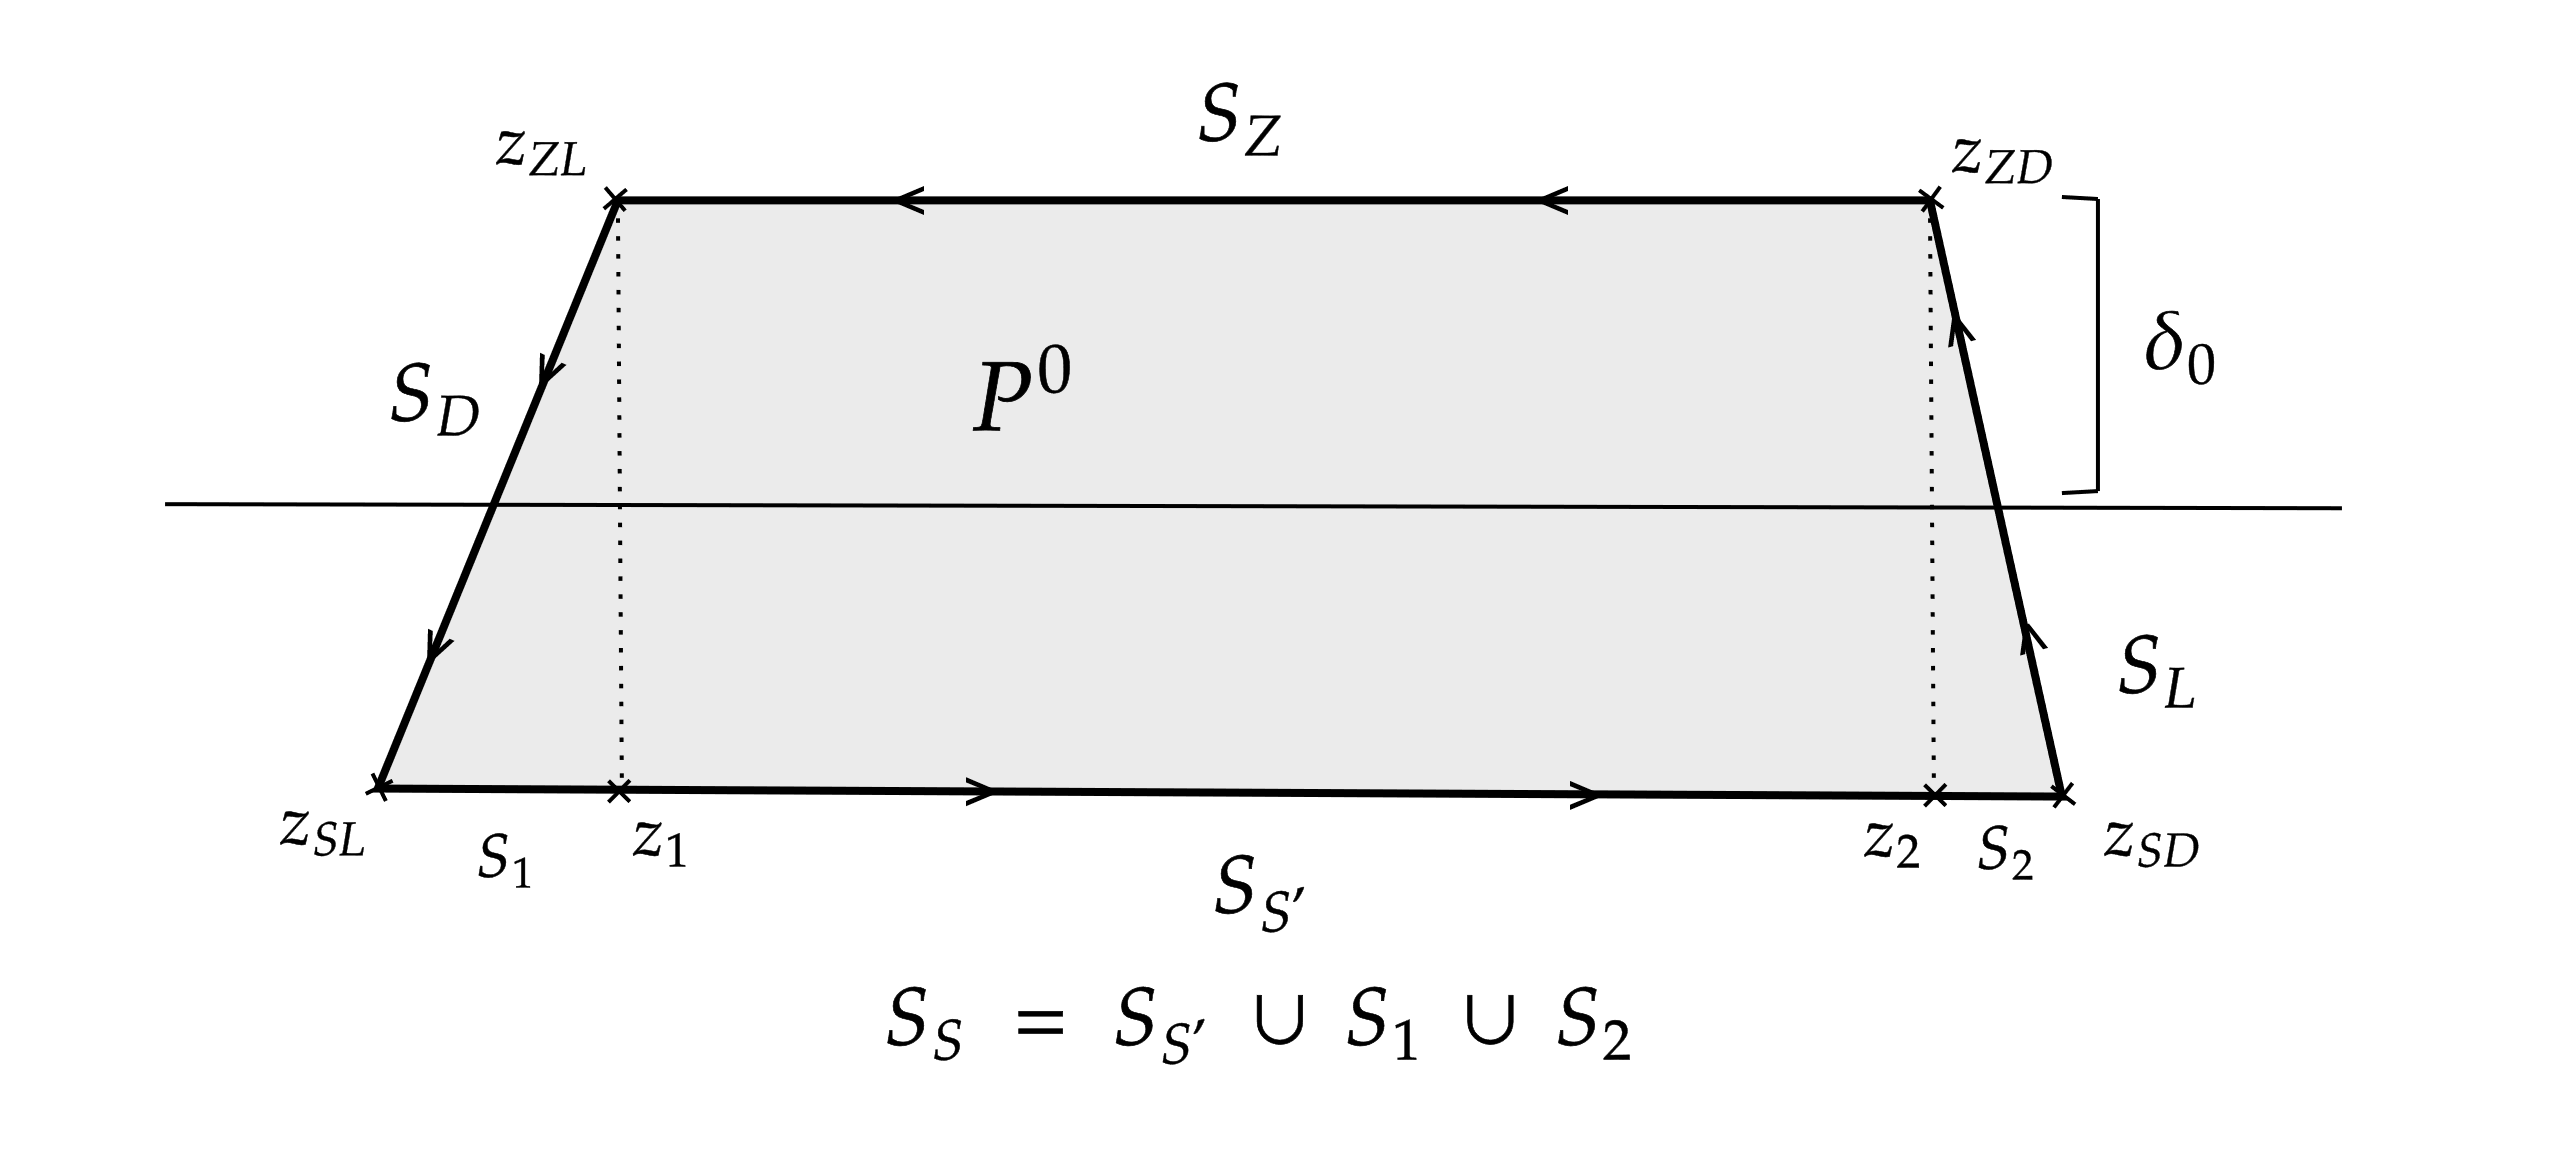
\includegraphics[width = \textwidth]{schwarz_hol_int.png}
                \caption{Delitev roba $P^0$ na $S_Z$, $S_D$, $S_L$ in $S_S$.}
            \end{center}    
        \end{figure}
        Sedaj zapisano delitev roba uporabimo pri zapisu krivuljnega integrala. Velja
        \begin{align*}
            \left|\int_{\partial P^0}{F(\xi)~d\xi}\right| &= \left|\int_{S_Z}{F(\xi)~d\xi} - \int_{S_S}{F(\xi)~d\xi} + \int_{S_L}{F(\xi)~d\xi} - \int_{S_D}{F(\xi)~d\xi}\right|\\
            & \leq \left|\int_{S_Z}{F(\xi)~d\xi} - \int_{S_S}{F(\xi)~d\xi} \right| + \left|\int_{S_L}{F(\xi)~d\xi}\right| + \left|\int_{S_D}{F(\xi)~d\xi}\right|.\\
        \end{align*}
        Ker je funkcija $F$ zvezna na $D$ je $|F|$ na $S_L$ in $S_D$ omejena. 
        Sedaj uporabimo trikotniško neenakost za integral in omejenost funkcije $|F|$ na $S_L$ oziroma $S_D$. 
        Opazimo, da bo absolutna vrednost integrala poljubno majhna, če bo le dolžina daljic $S_L$ in $S_D$ dovolj majhna. 
        Dovolj je zahtevati, da bo vrednost $\delta_0$ dovolj majhna. 
        Zapišimo nekoliko natančneje. Obstaja $\delta_1 > 0$, da za $\delta_0 \leq \delta_1$ velja
        $$ 
        \left|\int_{S_L}{F(\xi)~d\xi}\right| < \frac{\epsilon}{5}~~~\text{in}~~~\left|\int_{S_D}{F(\xi)~d\xi}\right| < \frac{\epsilon}{5}.
        $$
        Podoben sklep lahko naredimo pri integralu $\int_{S_1}{F(\xi)~d\xi}$ in $\int_{S_2}{F(\xi)~d\xi}$. Obstaja torej $\delta_2 > 0$, da za $\delta_0 \leq \delta_2$ velja
        $$ 
        \left|\int_{S_1}{F(\xi)~d\xi}\right| < \frac{\epsilon}{5}~~~\text{in}~~~\left|\int_{S_2}{F(\xi)~d\xi}\right| < \frac{\epsilon}{5}.
        $$
        Ko uporabimo zgornje ocene dobimo
        \begin{align*}
            \left|\int_{\partial P^0}{F(\xi)~d\xi}\right|&< \left|\int_{S_Z}{F(\xi)~d\xi} - \int_{S_{S'}}{F(\xi)~d\xi} - \int_{S_1}{F(\xi)~d\xi} - \int_{S_2}{F(\xi)~d\xi}\right| + \frac{\epsilon}{5} +  \frac{\epsilon}{5}\\
            & \leq \left|\int_{S_Z}{F(\xi)~d\xi} - \int_{S_{S'}}{F(\xi)~d\xi}\right| + \left|\int_{S_1}{F(\xi)~d\xi}\right| + \left|\int_{S_2}{F(\xi)~d\xi}\right| + \frac{2\epsilon}{5}\\
            & < \left|\int_{S_Z}{F(\xi_Z)~d\xi_Z} - \int_{S_{S'}}{F(\xi_{S'})~d\xi_{S'}}\right| + \frac{4\epsilon}{5}.\\
        \end{align*}
        Sedaj preostala integrala parametrizirajmo z $\xi_Z = (1 -t)z_{ZD} + t z_{ZL},~t \in [0,1]$ in $\xi_{S'} = (1 -t)z_{Z2} + t z_{Z1},~t \in [0,1]$.
        Sledi
        \begin{align*}
            &\int_{S_Z}{F(\xi_Z)~d\xi_Z} - \int_{S_{S'}}{F(\xi_{S'})~d\xi_{S'}}\\
            &=\int_{0}^{1}{F((1 -t)z_{ZD} + t z_{ZL})(z_{ZL} - z_{ZD})~dt} - \int_{0}^{1}{F((1 -t)z_{2} + t z_{1})(z_{1} - z_{2})~dt}\\
            &=\int_{0}^{1}{\left[F((1 -t)z_{ZD} + t z_{ZL})(z_{ZL} - z_{ZD}) - F((1 -t)z_{2} + t z_{1})(z_{1} - z_{2})\right]dt}.
        \end{align*}  
        Ker velja $z_{ZL} = z_{1} + 2 \delta_0$ in $z_{ZD} = z_2 + 2 \delta_0$ lahko zapišemo
        \begin{align*}
            &\int_{S_Z}{F(\xi_Z)~d\xi_Z} - \int_{S_{S'}}{F(\xi_{S'})~d\xi_{S'}}\\
            &=(z_{1} - z_{2})\int_{0}^{1}{\left[F((1 -t)z_{2} + t z_{1} + 2 \delta_0) - F((1 -t)z_{2} + t z_{1})\right]dt}.
        \end{align*}  
        Ker je $F$ zvezna na kompaktu $P^0$ obstaja $\delta_3 >0$, da za vsak $z, w \in P^0$ iz $|z -w| < \delta_3$ sledi $|F(z) - F(w)| < \frac{\epsilon}{5(z_1 - z_2)}$.
        Zato za $\delta_0 \leq \frac{\delta_3}{2}$ velja
        \begin{align*}
            &\left|\int_{S_Z}{F(\xi_Z)~d\xi_Z} - \int_{S_{S'}}{F(\xi_{S'})~d\xi_{S'}}\right|
            \leq (z_{1} - z_{2})\int_{0}^{1}{\frac{\epsilon}{5(z_{1} - z_{2})}~dt} < \frac{\epsilon}{5}.
        \end{align*}  
        Sedaj ocene združimo. Vzemimo $\delta_0 = \text{min}\{\delta_1, \delta_2, \frac{\delta_3}{2}\}$. Velja
        $$ 
        \left|\int_{\partial P^0}{F(\xi)~d\xi}\right|< \epsilon.
        $$
        Ker je bil $\epsilon$ poljubno majhen, iz tega že sledi $\int_{\partial T}{F(\xi)~d\xi} = 0$. 
        Da bo enakost veljala za vsak zaprt trikotnik iz okolice točke $z_0$, lahko namesto $\delta$ pri definiciji okolice vzamemo $\widetilde{\delta} = \delta_0 < \delta$. 
        Sledi, da je $F$ holomorfna na $\mathbb{D}(z_0, \widetilde{\delta})$. Ker je bil $z_0 \in D^0$ poljuben, smo dokazali, da je $F$ holomorfna tudi v okolici vsake točke iz $D^0$. 
    \end{dokaz}

\section{Zaključek}
    Pri formulaciji in dokazu Schwarzovega principa zrcaljenja smo razširitev iskali na zrcalni sliki območja glede na realno os. 
    Odsek realne osi, ki leži znotraj našega območja, bi lahko seveda tudi parametrizirali in ga obravnavali kot krivuljo. 
    Seveda je tu krivulja, ki določa odsek realne osi dokaj preprosta in zato obvladljiva.
    Iz tega vidika smo podano harmonično oziroma holomorfno funkcijo eksplicitno razširili na območje prek obvladljive krivulje.
    Prav takšen pristop nas vodi k posplošitvi Schwarzovega principa zrcaljenja. 
    Ta nam omogoča razširitev oziroma zrcaljenje podane funkcije tudi čez druge obvladljive krivulje. 
    Natančno formulacijo omenjenega izreka, ki odgovori tudi na vprašanje kaj točno je zgoraj skrito za besedami obvladljiva krivulja, si bralec lahko ogleda v REF GAM ali v REF DRUGA.

\bibliographystyle{siam}
\begin{thebibliography}{9}
    \bibitem{osnova}
    Theodore W. Gamelin \emph{Complex Analysis}, Springer (2001), Chapter X, str. 274 - 288

    \bibitem{mean value p}
    Weisstein, Eric W. \emph{Mean-Value Property}, v: From MathWorld--A Wolfram Web Resource, [ogled 22. 2. 2023], dostopno na
\end{thebibliography}

\end{document}